%% bare_jrnl.tex
%% V1.3
%% 2007/01/11
%% by Michael Shell
%% see http://www.michaelshell.org/
%% for current contact information.
%%
%% This is a skeleton file demonstrating the use of IEEEtran.cls
%% (requires IEEEtran.cls version 1.7 or later) with an IEEE journal paper.
%%
%% Support sites:
%% http://www.michaelshell.org/tex/ieeetran/
%% http://www.ctan.org/tex-archive/macros/latex/contrib/IEEEtran/
%% and
%% http://www.ieee.org/



% *** Authors should verify (and, if needed, correct) their LaTeX system  ***
% *** with the testflow diagnostic prior to trusting their LaTeX platform ***
% *** with production work. IEEE's font choices can trigger bugs that do  ***
% *** not appear when using other class files.                            ***
% The testflow support page is at:
% http://www.michaelshell.org/tex/testflow/


%%*************************************************************************
%% Legal Notice:
%% This code is offered as-is without any warranty either expressed or
%% implied; without even the implied warranty of MERCHANTABILITY or
%% FITNESS FOR A PARTICULAR PURPOSE! 
%% User assumes all risk.
%% In no event shall IEEE or any contributor to this code be liable for
%% any damages or losses, including, but not limited to, incidental,
%% consequential, or any other damages, resulting from the use or misuse
%% of any information contained here.
%%
%% All comments are the opinions of their respective authors and are not
%% necessarily endorsed by the IEEE.
%%
%% This work is distributed under the LaTeX Project Public License (LPPL)
%% ( http://www.latex-project.org/ ) version 1.3, and may be freely used,
%% distributed and modified. A copy of the LPPL, version 1.3, is included
%% in the base LaTeX documentation of all distributions of LaTeX released
%% 2003/12/01 or later.
%% Retain all contribution notices and credits.
%% ** Modified files should be clearly indicated as such, including  **
%% ** renaming them and changing author support contact information. **
%%
%% File list of work: IEEEtran.cls, IEEEtran_HOWTO.pdf, bare_adv.tex,
%%                    bare_conf.tex, bare_jrnl.tex, bare_jrnl_compsoc.tex
%%*************************************************************************

% Note that the a4paper option is mainly intended so that authors in
% countries using A4 can easily print to A4 and see how their papers will
% look in print - the typesetting of the document will not typically be
% affected with changes in paper size (but the bottom and side margins will).
% Use the testflow package mentioned above to verify correct handling of
% both paper sizes by the user's LaTeX system.
%
% Also note that the "draftcls" or "draftclsnofoot", not "draft", option
% should be used if it is desired that the figures are to be displayed in
% draft mode.
%
\documentclass[journal]{IEEEtran}
\usepackage[table]{xcolor}
%
% If IEEEtran.cls has not been installed into the LaTeX system files,
% manually specify the path to it like:
% \documentclass[journal]{../sty/IEEEtran}





% Some very useful LaTeX packages include:
% (uncomment the ones you want to load)


% *** MISC UTILITY PACKAGES ***
%
%\usepackage{ifpdf}
% Heiko Oberdiek's ifpdf.sty is very useful if you need conditional
% compilation based on whether the output is pdf or dvi.
% usage:
% \ifpdf
%   % pdf code
% \else
%   % dvi code
% \fi
% The latest version of ifpdf.sty can be obtained from:
% http://www.ctan.org/tex-archive/macros/latex/contrib/oberdiek/
% Also, note that IEEEtran.cls V1.7 and later provides a builtin
% \ifCLASSINFOpdf conditional that works the same way.
% When switching from latex to pdflatex and vice-versa, the compiler may
% have to be run twice to clear warning/error messages.



%\usepackage[table]{xcolor}

\usepackage{comment}
\usepackage{array}
\usepackage{caption}
%\usepackage[dvipsnames]{xcolor}
%\usepackage[dvipsnames]{xcolor}

%\usepackage{lipsum}
%\usepackage{color}
%\usepackage{colortbl}
%\usepackage[table]{xcolor}
%\definecolor{orange}{rgb}{1,0.647,0}
%\definecolor{Gray}{gray}{0.65}
%\definecolor{Blue}{RGB}{0,176,240}
%\definecolor{light-gray}{gray}{0.90}

% *** CITATION PACKAGES ***
%
%\usepackage{natbib}
\usepackage{cite}
%\usepackage{subcaption}
% cite.sty was written by Donald Arseneau
% V1.6 and later of IEEEtran pre-defines the format of the cite.sty package
% \cite{} output to follow that of IEEE. Loading the cite package will
% result in citation numbers being automatically sorted and properly
% "compressed/ranged". e.g., [1], [9], [2], [7], [5], [6] without using
% cite.sty will become [1], [2], [5]--[7], [9] using cite.sty. cite.sty's
% \cite will automatically add leading space, if needed. Use cite.sty's
% noadjust option (cite.sty V3.8 and later) if you want to turn this off.
% cite.sty is already installed on most LaTeX systems. Be sure and use
% version 4.0 (2003-05-27) and later if using hyperref.sty. cite.sty does
% not currently provide for hyperlinked citations.
% The latest version can be obtained at:
% http://www.ctan.org/tex-archive/macros/latex/contrib/cite/
% The documentation is contained in the cite.sty file itself.






% *** GRAPHICS RELATED PACKAGES ***
%
\ifCLASSINFOpdf
   \usepackage[pdftex]{graphicx}
  % declare the path(s) where your graphic files are
  % \graphicspath{{../pdf/}{../jpeg/}}
  % and their extensions so you won't have to specify these with
  % every instance of \includegraphics
  % \DeclareGraphicsExtensions{.pdf,.jpeg,.png}
\else
  % or other class option (dvipsone, dvipdf, if not using dvips). graphicx
  % will default to the driver specified in the system graphics.cfg if no
  % driver is specified.
   \usepackage[dvips]{graphicx}
  % declare the path(s) where your graphic files are
  % \graphicspath{{../eps/}}
  % and their extensions so you won't have to specify these with
  % every instance of \includegraphics
  % \DeclareGraphicsExtensions{.eps}
\fi
% graphicx was written by David Carlisle and Sebastian Rahtz. It is
% required if you want graphics, photos, etc. graphicx.sty is already
% installed on most LaTeX systems. The latest version and documentation can
% be obtained at: 
% http://www.ctan.org/tex-archive/macros/latex/required/graphics/
% Another good source of documentation is "Using Imported Graphics in
% LaTeX2e" by Keith Reckdahl which can be found as epslatex.ps or
% epslatex.pdf at: http://www.ctan.org/tex-archive/info/
%
% latex, and pdflatex in dvi mode, support graphics in encapsulated
% postscript (.eps) format. pdflatex in pdf mode supports graphics
% in .pdf, .jpeg, .png and .mps (metapost) formats. Users should ensure
% that all non-photo figures use a vector format (.eps, .pdf, .mps) and
% not a bitmapped formats (.jpeg, .png). IEEE frowns on bitmapped formats
% which can result in "jaggedy"/blurry rendering of lines and letters as
% well as large increases in file sizes.
%
% You can find documentation about the pdfTeX application at:
% http://www.tug.org/applications/pdftex



\usepackage{tikz}
\usetikzlibrary{arrows.meta,shapes,shadows,arrows,decorations.pathreplacing,decorations.markings}
\usepackage{longtable}
\usepackage{tabularx}
\usepackage{multicol}

% *** MATH PACKAGES ***
%
\usepackage[cmex10]{amsmath}
% A popular package from the American Mathematical Society that provides
% many useful and powerful commands for dealing with mathematics. If using
% it, be sure to load this package with the cmex10 option to ensure that
% only type 1 fonts will utilized at all point sizes. Without this option,
% it is possible that some math symbols, particularly those within
% footnotes, will be rendered in bitmap form which will result in a
% document that can not be IEEE Xplore compliant!
%
% Also, note that the amsmath package sets \interdisplaylinepenalty to 10000
% thus preventing page breaks from occurring within multiline equations. Use:
%\interdisplaylinepenalty=2500
% after loading amsmath to restore such page breaks as IEEEtran.cls normally
% does. amsmath.sty is already installed on most LaTeX systems. The latest
% version and documentation can be obtained at:
% http://www.ctan.org/tex-archive/macros/latex/required/amslatex/math/





% *** SPECIALIZED LIST PACKAGES ***
%
%\usepackage{algorithmic}
% algorithmic.sty was written by Peter Williams and Rogerio Brito.
% This package provides an algorithmic environment fo describing algorithms.
% You can use the algorithmic environment in-text or within a figure
% environment to provide for a floating algorithm. Do NOT use the algorithm
% floating environment provided by algorithm.sty (by the same authors) or
% algorithm2e.sty (by Christophe Fiorio) as IEEE does not use dedicated
% algorithm float types and packages that provide these will not provide
% correct IEEE style captions. The latest version and documentation of
% algorithmic.sty can be obtained at:
% http://www.ctan.org/tex-archive/macros/latex/contrib/algorithms/
% There is also a support site at:
% http://algorithms.berlios.de/index.html
% Also of interest may be the (relatively newer and more customizable)
% algorithmicx.sty package by Szasz Janos:
% http://www.ctan.org/tex-archive/macros/latex/contrib/algorithmicx/




% *** ALIGNMENT PACKAGES ***
%
\usepackage{array}
% Frank Mittelbach's and David Carlisle's array.sty patches and improves
% the standard LaTeX2e array and tabular environments to provide better
% appearance and additional user controls. As the default LaTeX2e table
% generation code is lacking to the point of almost being broken with
% respect to the quality of the end results, all users are strongly
% advised to use an enhanced (at the very least that provided by array.sty)
% set of table tools. array.sty is already installed on most systems. The
% latest version and documentation can be obtained at:
% http://www.ctan.org/tex-archive/macros/latex/required/tools/


%\usepackage{mdwmath}
%\usepackage{mdwtab}
% Also highly recommended is Mark Wooding's extremely powerful MDW tools,
% especially mdwmath.sty and mdwtab.sty which are used to format equations
% and tables, respectively. The MDWtools set is already installed on most
% LaTeX systems. The lastest version and documentation is available at:
% http://www.ctan.org/tex-archive/macros/latex/contrib/mdwtools/


% IEEEtran contains the IEEEeqnarray family of commands that can be used to
% generate multiline equations as well as matrices, tables, etc., of high
% quality.


\usepackage{eqparbox}
% Also of notable interest is Scott Pakin's eqparbox package for creating
% (automatically sized) equal width boxes - aka "natural width parboxes".
% Available at:
% http://www.ctan.org/tex-archive/macros/latex/contrib/eqparbox/





% *** SUBFIGURE PACKAGES ***
\usepackage[tight,footnotesize]{subfigure}
% subfigure.sty was written by Steven Douglas Cochran. This package makes it
% easy to put subfigures in your figures. e.g., "Figure 1a and 1b". For IEEE
% work, it is a good idea to load it with the tight package option to reduce
% the amount of white space around the subfigures. subfigure.sty is already
% installed on most LaTeX systems. The latest version and documentation can
% be obtained at:
% http://www.ctan.org/tex-archive/obsolete/macros/latex/contrib/subfigure/
% subfigure.sty has been superceeded by subfig.sty.



%\usepackage[caption=false]{caption}
%\usepackage[font=footnotesize]{subfig}
% subfig.sty, also written by Steven Douglas Cochran, is the modern
% replacement for subfigure.sty. However, subfig.sty requires and
% automatically loads Axel Sommerfeldt's caption.sty which will override
% IEEEtran.cls handling of captions and this will result in nonIEEE style
% figure/table captions. To prevent this problem, be sure and preload
% caption.sty with its "caption=false" package option. This is will preserve
% IEEEtran.cls handing of captions. Version 1.3 (2005/06/28) and later 
% (recommended due to many improvements over 1.2) of subfig.sty supports
% the caption=false option directly:
%\usepackage[caption=false,font=footnotesize]{subfig}
%
% The latest version and documentation can be obtained at:
% http://www.ctan.org/tex-archive/macros/latex/contrib/subfig/
% The latest version and documentation of caption.sty can be obtained at:
% http://www.ctan.org/tex-archive/macros/latex/contrib/caption/




% *** FLOAT PACKAGES ***
%
%\usepackage{fixltx2e}
% fixltx2e, the successor to the earlier fix2col.sty, was written by
% Frank Mittelbach and David Carlisle. This package corrects a few problems
% in the LaTeX2e kernel, the most notable of which is that in current
% LaTeX2e releases, the ordering of single and double column floats is not
% guaranteed to be preserved. Thus, an unpatched LaTeX2e can allow a
% single column figure to be placed prior to an earlier double column
% figure. The latest version and documentation can be found at:
% http://www.ctan.org/tex-archive/macros/latex/base/



\usepackage{stfloats}
% stfloats.sty was written by Sigitas Tolusis. This package gives LaTeX2e
% the ability to do double column floats at the bottom of the page as well
% as the top. (e.g., "\begin{figure*}[!b]" is not normally possible in
% LaTeX2e). It also provides a command:
%\fnbelowfloat
% to enable the placement of footnotes below bottom floats (the standard
% LaTeX2e kernel puts them above bottom floats). This is an invasive package
% which rewrites many portions of the LaTeX2e float routines. It may not work
% with other packages that modify the LaTeX2e float routines. The latest
% version and documentation can be obtained at:
% http://www.ctan.org/tex-archive/macros/latex/contrib/sttools/
% Documentation is contained in the stfloats.sty comments as well as in the
% presfull.pdf file. Do not use the stfloats baselinefloat ability as IEEE
% does not allow \baselineskip to stretch. Authors submitting work to the
% IEEE should note that IEEE rarely uses double column equations and
% that authors should try to avoid such use. Do not be tempted to use the
% cuted.sty or midfloat.sty packages (also by Sigitas Tolusis) as IEEE does
% not format its papers in such ways.


%\ifCLASSOPTIONcaptionsoff
%  \usepackage[nomarkers]{endfloat}
% \let\MYoriglatexcaption\caption
% \renewcommand{\caption}[2][\relax]{\MYoriglatexcaption[#2]{#2}}
%\fi
% endfloat.sty was written by James Darrell McCauley and Jeff Goldberg.
% This package may be useful when used in conjunction with IEEEtran.cls'
% captionsoff option. Some IEEE journals/societies require that submissions
% have lists of figures/tables at the end of the paper and that
% figures/tables without any captions are placed on a page by themselves at
% the end of the document. If needed, the draftcls IEEEtran class option or
% \CLASSINPUTbaselinestretch interface can be used to increase the line
% spacing as well. Be sure and use the nomarkers option of endfloat to
% prevent endfloat from "marking" where the figures would have been placed
% in the text. The two hack lines of code above are a slight modification of
% that suggested by in the endfloat docs (section 8.3.1) to ensure that
% the full captions always appear in the list of figures/tables - even if
% the user used the short optional argument of \caption[]{}.
% IEEE papers do not typically make use of \caption[]'s optional argument,
% so this should not be an issue. A similar trick can be used to disable
% captions of packages such as subfig.sty that lack options to turn off
% the subcaptions:
% For subfig.sty:
% \let\MYorigsubfloat\subfloat
% \renewcommand{\subfloat}[2][\relax]{\MYorigsubfloat[]{#2}}
% For subfigure.sty:
% \let\MYorigsubfigure\subfigure
% \renewcommand{\subfigure}[2][\relax]{\MYorigsubfigure[]{#2}}
% However, the above trick will not work if both optional arguments of
% the \subfloat/subfig command are used. Furthermore, there needs to be a
% description of each subfigure *somewhere* and endfloat does not add
% subfigure captions to its list of figures. Thus, the best approach is to
% avoid the use of subfigure captions (many IEEE journals avoid them anyway)
% and instead reference/explain all the subfigures within the main caption.
% The latest version of endfloat.sty and its documentation can obtained at:
% http://www.ctan.org/tex-archive/macros/latex/contrib/endfloat/
%
% The IEEEtran \ifCLASSOPTIONcaptionsoff conditional can also be used
% later in the document, say, to conditionally put the References on a 
% page by themselves.





% *** PDF, URL AND HYPERLINK PACKAGES ***
%
\usepackage{url}
% url.sty was written by Donald Arseneau. It provides better support for
% handling and breaking URLs. url.sty is already installed on most LaTeX
% systems. The latest version can be obtained at:
% http://www.ctan.org/tex-archive/macros/latex/contrib/misc/
% Read the url.sty source comments for usage information. Basically,
% \url{my_url_here}.





% *** Do not adjust lengths that control margins, column widths, etc. ***
% *** Do not use packages that alter fonts (such as pslatex).         ***
% There should be no need to do such things with IEEEtran.cls V1.6 and later.
% (Unless specifically asked to do so by the journal or conference you plan
% to submit to, of course. )


% correct bad hyphenation here
\hyphenation{op-tical net-works semi-conduc-tor}

\pagestyle{empty}
\usepackage{amsmath}
%\usepackage{mdwtab}
\usepackage{multirow}
% \usepackage[pdftex]{graphicx}
%\usetikzlibrary{matrix,shapes,arrows,positioning,chains}
\usetikzlibrary{shapes,arrows}
\begin{document}
%
% paper title
% can use linebreaks \\ within to get better formatting as desired
\title{THEORITICAL PREDICTION AND MATHEMATICAL FORMUALTION OF THE MATERIAL  COMPOSITION FOR MICROWAVE ABSORPTION APPLICATIONS}
%
%
% author names and IEEE memberships
% note positions of commas and nonbreaking spaces ( ~ ) LaTeX will not break
% a structure at a ~ so this keeps an author's name from being broken across
% two lines.
% use \thanks{} to gain access to the first footnote area
% a separate \thanks must be used for each paragraph as LaTeX2e's \thanks
% was not built to handle multiple paragraphs
%

\author{Aayushi Arya,Dr GVV Sharma}
%,~\IEEEmembership{Member,~IEEE,}
 %      John~Doe,~\IEEEmembership{Fellow,~OSA,}
  %    and~Jane~Doe,~\IEEEmembership{Life~Fellow,~IEEE}% <-this % stops a space
%  \author{AayushiArya}
%\thanks{M. Shell is with the Department
%of Electrical and Computer Engineering, Georgia Institute of Technology, Atlanta,
%GA, 30332 USA e-mail: (see http://www.michaelshell.org/contact.html).}% <-this % stops a space
%\thanks{J. Doe and J. Doe are with Anonymous University.}% <-this % stops a space
%\thanks{Manuscript received April 19, 2005; revised January 11, 2007.}}

% note the % following the last \IEEEmembership and also \thanks - 
% these prevent an unwanted space from occurring between the last author name
% and the end of the author line. i.e., if you had this:
% 
% \author{....lastname \thanks{...} \thanks{...} }
%                     ^------------^------------^----Do not want these spaces!
%
% a space would be appended to the last name and could cause every name on that
% line to be shifted left slightly. This is one of those "LaTeX things". For
% instance, "\textbf{A} \textbf{B}" will typeset as "A B" not "AB". To get
% "AB" then you have to do: "\textbf{A}\textbf{B}"
% \thanks is no different in this regard, so shield the last } of each \thanks
% that ends a line with a % and do not let a space in before the next \thanks.
% Spaces after \IEEEmembership other than the last one are OK (and needed) as
% you are supposed to have spaces between the names. For what it is worth,
% this is a minor point as most people would not even notice if the said evil
% space somehow managed to creep in.



% The paper headers
\markboth{Journal of \LaTeX\ Class Files,~Vol.~6, No.~1, January~2007}%
{Shell \MakeLowercase{\textit{et al.}}: Bare Demo of IEEEtran.cls for Journals}
% The only time the second header will appear is for the odd numbered pages
% after the title page when using the twoside option.
% 
% *** Note that you probably will NOT want to include the author's ***
% *** name in the headers of peer review papers.                   ***
% You can use \ifCLASSOPTIONpeerreview for conditional compilation here if
% you desire.




% If you want to put a publisher's ID mark on the page you can do it like
% this:
%\IEEEpubid{0000--0000/00\$00.00~\copyright~2007 IEEE}
% Remember, if you use this you must call \IEEEpubidadjcol in the second
% column for its text to clear the IEEEpubid mark.



% use for special paper notices
%\IEEEspecialpapernotice{(Invited Paper)}



\maketitle
\thispagestyle{empty}


\begin{abstract}
%\boldmath
Microwave Absorbers has become an essential requirement in various fields including industrial uses like Radar, Stealth , commercial uses in mobile networking , EMI , EMC, electronic toll collection, social applications like in hospitals , schools , where the microwave flux has crossed the threshold. In the past few years, there has been  an intense experimental work to explore various materials for the different applications , focusssing on their effectiveness, stability. The hit and trial cycles of the experimentation can be reduced with a theoritical model predicting the suitability of material for MA applications, allowing more accurate , rigorous and wide prespective for the experimentation. Thus, in this work , an attempt has been made provide a conceptual and theoritical mathematical formulation based model to predict the suitability of various elements and their composition for specified application. The model is based on Transmission Line Theory, Polarizability, dielectric response of material. The  parameters are derived for the MA  are characteristic impedance, input impedance , permittivity , permeability polarizability , Molar refraction ratio, Polarisation Energy. Using the above paramters and the material properties like its global hardness factor, we conclude to a set of theoritical atomic radii , which can be suitable for the absorption at the specified frequency , which is 2.54 GHz ( ISM band -immensely used in various eelctronic applications). Further a composition of two or more elements viz. oxides of material, alloys , and multi cation oxides, can be predicted by comparing their spatial energy parameter , which depends on their individual valency and global hardness factor.This work is beneficial for not only understanding the fundamental molecular level perspective of the absorbers but also in providing a conceptual and engineering aspect to further explore new materials for the microwave absorption , with less error rate.
\end{abstract}
% IEEEtran.cls defaults to using nonbold math in the Abstract.
% This preserves the distinction between vectors and scalars. However,
% if the journal you are submitting to favors bold math in the abstract,
% then you can use LaTeX's standard command \boldmath at the very start
% of the abstract to achieve this. Many IEEE journals frown on math
% in the abstract anyway.

% Note that keywords are not normally used for peerreview papers.
\begin{IEEEkeywords}
EMI , Reflection Loss, Resonance, Dielectric Parameters,Polarisation Energy,Atomic Radii.
\end{IEEEkeywords}






% For peer review papers, you can put extra information on the cover
% page as needed:
% \ifCLASSOPTIONpeerreview
% \begin{center} \bfseries EDICS Category: 3-BBND \end{center}
% \fi
%
% For peerreview papers, this IEEEtran command inserts a page break and
% creates the second title. It will be ignored for other modes.
\IEEEpeerreviewmaketitle



\section{Introduction}
% The very first letter is a 2 line initial drop letter followed
% by the rest of the first word in caps.
% 
% form to use if the first word consists of a single letter:
% \IEEEPARstart{A}{demo} file is ....
% 
% form to use if you need the single drop letter followed by
% normal text (unknown if ever used by IEEE):
% \IEEEPARstart{A}{}demo file is ....
% 
% Some journals put the first two words in caps:
% \IEEEPARstart{T}{his demo} file is ....
% 
% Here we have the typical use of a "T" for an initial drop letter
% and "HIS" in caps to complete the first word.
\IEEEPARstart{M}{icrowave Absorbers} , has now become an area of  immense research for both electronic field and materials design . The immediate need of Microwave absorbers is highlighted due to their necessity in the current technological scenario. need Due to the exponential growth of the usage of high frequency  electronic hardware and wireless communication, there is a dramatical increase of the microwaves flux in the ambient surroundings , which causes ElectroMagnetic Interference amomg the underlying circuits undesirably by generating unwanted noise, cross connection ,false output etc\cite{Shukla}. The critical exposure of microwaves  also has harmful effects on the health , especially for hospitals, schools and highly populated residential areas. This creates a  need to mitigate the surrounding EM wave  noise, has driven researchers to develop materials that can effectively absorb the unwanted radiations ,protecting the underneath circuitry\cite{r14}. Various materials and their composition are investigated using experimental procedures like Vector Network Analyzer, Impedance Analyzer to test their ability as absorbers. With new type of materials including pervoskites, oxides , ferrites and ,metamaterials being explored for absoption application owing to their enhanced physical and chemical stability, there is a need to theoritically understand the complex fundamentals for the working of an efficient Microwave Absorber. There  has been work  work to theoritically understand and model the wave parameters of Microwave Absorbers\cite{YingL2,YingL} based on transmission Line Theory.There has been also works to correlate the electrical/magnetic parameter and physical parameters of microwave absorbers. Analyising polarizability gives an insight into the wave absorbing power of a material. Following this , in \cite{Erbium} , the Lorentz-Lorenz equation was used to estimate  the electronic polarizability of ions in oxide glasses , based on their refractive indices and band gap energy.In \cite{JaiS} Polarizability behaviour for transition metal oxides have also been studied and a relationship between their atomic radii and polarizability have been developed .In \cite{dimitrov1999effect,dimitrov1999electronic} , the author further discusses an Interaction Parameter for oxides based  on the polarizability of oxide ion, dtermined from the refractive index. This Parameter is used as a measure of the interionic interaction between cations and anions created due to the charge overlap of the outermost electronic orbitals.The charge overlap and the polarizability of cation and anions both affect the Interaction Parameter.
% This Parameter serves as an index to estimate the optical  properties of oxide glasses. Siimilarly for magnetic based microwave absorbers the magnetic dipole moment can be used as a measure for microwave absprtion.  This consecutive dependency of  properties when modelled mathematically using energy parmeter can provide a useful tool for prediction of new compositions based suitable microwave absorbing materials.
The energy parameter when normalized can be directly related to the atomic radii \cite{korablev2018calculations}. There are range of wave theory based electrical, magnetic parameters associated with the working of MA. Magnetic Microwave Absorbers are also evaluated and studied for their underlying phenomenons. In  \cite{liu2018systemized} a theory is developed for ferrite based microwave absorbers conatining both electric and magnetic dipoles represnted by  permittivity and permeability respectively. In \cite{patil1985susceptibility} mathematical  relationships have been shown  between magnetic susceptibility and polarizability of atoms using ionization energy. The work shows proportionality between the susceptibility and polarizability with the proportionality constant being the total number of electrons and atomic number.

Similar theory is applicable to ferrite based microwave absorbers conatining both electric and magnetic dipoles represnted by  permittivity and permeability respectively \cite{liu2018systemized}.The oscillations of dipoles in a MA are both resonant and non resonant . A detailed absorption model is then provided to include all the above elements in the basics of absorption formulas of transmission line theory.
In this paper , an attempt has been made to theoritically predict the atomic and physical properties of a microwave absorber from its electrcical and magnetic properties. It presents a unique approach of calculating the fundamental parameters of an absorber by establishing relationship between the various phenomenon of an absorber and suggest a theoritical model to predict and analyse the potential material composition for an effective microwave absorber.
%In this paper, an attempt has been made to theoritically derive the parameter related to a microwave absorber. First the transmission line theory was used to determine the electrical parameters including characteristic impedance, reflection loss, permittivity and permeability, resonance frequency . From the above paremters and a set of equations expalined below we derived  the physical parameters like polarizability, dipolar frequency . spatial energy parameter . From this we derived   the atomic range of suitable atomic radii . The compositions can be predicted by comparing the effective Energy Parameter. This approach covers all the necessary  properties required for a microwave absorber. It can be beneficial in filling the gap between the molecular and the physical properties of an absorber . It can help in predicting new compositions for efficient microwave absorbption.
%\newline
%\Large{

\begin{table*}[t]
%	\centering
	
	
	%\resizebox{\textwidth}{!}{
	%	\begin{table}
	%\begin{flushleft}
	
	
	%\begin{figure*}
	%\resizebox{0.5\textwidth}{!}{
	%\begin{table}[!ht]
	
	%\begin{table}
	\caption{Constant values}
	\label{1}
	
	\begin{tabular}{|c|c|c|c|}
		\hline 
		Constant & \multicolumn{2}{|l|}{Description} & Value \\ 
		\hline
		R.L & \multicolumn{2}{|l|}{Reflection Loss} &-20 dB \\
		\hline
		
		${Z_{o}}_{free}$ & \multicolumn{2}{|l|}{Characteristic Impedance of Free Space} & 377 $\Omega$ \\
		\hline
		$f_r$ & \multicolumn{2}{|l|}{Resonance Frequency} & 2.54GHz \\
		\hline
		$\zeta$ &\multicolumn{2}{|l|}{ Damping Factor} & 1.5 \\
		\hline
		$\triangle f_r$ & \multicolumn{2}{|l|}{Bandwidth} & 7.7 GHz \\
		\hline
		$\omega_r$ & \multicolumn{2}{|l|}{angular resonance frequency} & $ 1.53x10^{10} rad/sec$ \\
		\hline
		$\omega_r$ & \multicolumn{2}{|l|}{angular bandwidth } & $ 4.83x10^{10} rad/sec$ \\
		\hline
		$\omega$ &\multicolumn{2}{|l|}{ Upper frequency limit}  & $5 x 10^{10} rad/sec$ \\
		\hline
		A &\multirow{3}{*}{ Cauchy  dispersion}  & $A = 1+ {n_o}^2$ ,
		$n_o $ \tiny{=upper limit of refractive index }& 4.41\\
		\cline{1-1} \cline{3-4}
		B              &             &      $B = (2 \pi c)^2 \dfrac{\chi_e(0)}{{\omega_{oe}}^2}$     ,   $ {\omega_{oe}}^2 = \dfrac{{\omega_o}^2}{{n_o}^2}$    &      \\
		\cline{1-1} \cline{3-4}
		C              &              &    $C= \dfrac{B}{2 A^{1/2}}$              & $3.32x10^{-3}$       \\
		\cline{1-1} \cline{3-4}
		\hline
		$\mu_B$ & \multicolumn{2}{|l|}{Bohr Magneton } & $9.27 X 10^{-21} erg/ gauss$ (CGS unit) \\
		\hline
		$\mu_o$ &  \multicolumn{2}{|l|}{Free Space Permeability} &  $4 \pi X 10^{-7} Hm^{-1}$ \\
		\hline
		$\epsilon_o$ & \multicolumn{2}{|l|}{Free Space Permittivity} & $8.85 X 10^{-12} F m^{-1}$ \\
		\hline
		T & \multicolumn{2}{|l|}{ Absolute Temperature} & 300 K \\
		\hline
		m & \multicolumn{2}{|l|}{ Mass of electron} & $9.1 X 10 ^{-31} Kg $ \\
		\hline
		$k_B$ & \multicolumn{2}{|l|}{Boltzmann Constant } & $1.38 X 10 ^{-23} J.K^{-1}$ \\
		\hline
		N & \multicolumn{2}{|l|}{Avagadro Number } & $6.022 X 10 ^{23}$ \\
		\hline
		$q^2 /2 $ & \multicolumn{2}{|l|}{ratio of unit charge to energy in C.G.S unit} & $7.19 X 10^{-8}$ \\
		\hline
		$\eta_g$ & \multicolumn{2}{|l|}{Global Hardness Factor} & Ref. \cite{ghosh2002theoretical} \\
		\hline
	\end{tabular}
	% \end{figure*}
	%}
\end{table*}
%}
%}
%\end{longtable}

%	\end{figure*}
%\end{flushleft}
\subsection{Description of Theoritical Calculation}
A microwave absorber is characterised by its reflection Loss,resonance frequency and its bandwidth.  With the desired specifications of a Microwave Absorber, the electrical , magnetic and atomic parameters of the required  material composition can be found  using Transmission Line Theory, Polarizability, Electric and Magnetic Susceptibility\cite{YingL,liu2018systemized}.The transmission Line theory considers the absorber as a transmission line with its reflection loss being proportional to the input impedance . It also assigns a characteristic impedance to the absorber which is an  is an intrinsic property independent of the thickness of the absorber.The absorber also follows the quality factor and damping ratio as per the desired frequency and wavelength\cite{Cory,Tooley} Similarly the presence of electric energy loss can be understood with the polarization theory. The polarisability provides a means of charge separation and forming dipoles which dissipates the electric energy\cite{AlphaP,Inter}. Third is the magnetic loss phenomenon which follows the theory of formation of the magnetic dipoles \cite{}  .Using the different theories and relations flow chart \ref{f(a)} is shown with all the steps and equations that are used to evaluate the atomic parameters from the electrical and magnetic properties of the absorber. As shown in the following flow chart, the speifications available for absorbers are Reflection Loss, Resonance Frequency and Resonance Bandwidth. All the three depends on the application of use. Here the telecommunication frequency(ISM BAND) has been used as reference , which is widely used in most of the electronic and communication industry. There are three branches of the chart , one that uses Transmission Line Theory and goes from R.L to input impedance, charcteristic impedance and finaaly to the lower limit of refractive index \cite{YingL,Shukla} . The second follows polarization theory and deduces different parameters associated to polarization including wave propagation constant , polarizability, Number of dipoles using Claussius Mosotti equation \cite{liu2018systemized,shannon,Erbium,polar}. The third uses the complex permittivity values to obtain the upper limit of refractive index. The branches have interlinkings due to use of related parameters\cite{Ian,booke}. Finally using the formuala of calculating polarisation energy from the refraction ratio, the global Hardness Factor can be calculated which is a  measure of the extent of polarisation that a molecule can undergo\cite{ghosh2002theoretical}. Using it , the corresponding atomic radii can be calculated giving a range of lower and upper atomic radii which can be selected for use in the required Microwave Absorber.
\subsection{EFFECTIVE ENERGY PARAMETER}
From the range of calculated atomic radii , suitable material compositions can be found out by formualtion a way of comparing the compatibility of different elements towards each other based on their effective energy parameter\cite{korablev2018calculations}. This Parameter serves as a measure of the element's tendency to ionize. The parameter depends on the effective charge of nucleus , effective quantum number, gloabal hardness factor and atomic radii. The derivations for which are provided below. The effective quantum number was calculated from the orbital exponents of indiviadual elements divided by the their atomic number \cite{clementi1963atomic} .
For any compound , the effective energy parmeter is used to calculate the balance of the cations and anionic polarisation tendencies. If it is comparable. The compound will be suitable for Microwave Absorbption at desired frequency and bandwidth.
Using the effective energy parameter formulations are formed to predict the material compositions of microwave absorbers.  The materials considered here are oxides and ferrites.Flowchart \ref{f(b)} shows all the equations and formulae involved in calculating the effective energy parameter.
\subsection{MAGNETIC MICROWAVE ABSORBERS}
Magnetic microwave absorbers including ferrites and others have paved their way owing to the increased magnetic dissipation of energy along with the electrical energy dissipation\cite{HexaF}. In the coming section , a method has been suggested to calculate the magnetic dipole moments from the permeability value of the absorber, and providing a range of dipole moments suitabe for absorption application. The required magnetism in a compound depends on the difference of the cationic and anionic energy parameter. 
In a magnetic material based MA , there are additional magnetic losses along with the dielectric and ohmic losses. These are the losses due to magnetic resonance. The magnetic resonance is the result of the interaction between the magnetic field of the incident EM wave and the orbital as well as the spin angular momentum of the corresponding elements\cite{Ferrite}. When there is unpairing of the electrons in the outer orbital of the elements , there is an increase in the resultant magnetic moment, leading to enhanced magnetic losses\cite{HexaF} \cite{LaMn}. The magnetic losses can be accounted by the parameters like complex  permeability, susceptilbility, magnetic moment etc. for a specific element composition or a chemical compound.Using the proportionality betweeen the susceptibility and the polarizability of atoms \cite{patil1985susceptibility}, the lack of electric energy loss can be compensated by the magnetic losses in a magnetic microwave absorber leading to improved efficiency.
A difference is to be noted here for d-shell and f-shell magnetic materials.  Magnetic compounds like ferrites have quenched orbital angular momentum for d-shell magnetic materials by virtue of the  orbital angular momentum being tied to the Easy Magnetisation Direction (EMD). While in the f-fhell electrons, due to the asymmetrical nature of the orbitals, the orbital angular momentum exists, which is more dominant then the spin angular momentum \cite{mchenry2002magnetic}.
For the d-shell materials
Langevin's theory develops an analogy between dielectric and magnetic phenomenon,including the complex permittivity and permeability. Using the above theory,the magnetic losses in the d-shell and the f-shell elements can be associated to the imaginary part and real part of permeability respectively.The imaginary part of permeability is indicative of the dissipation of magnetic energy which  can be related to the spin angular moment caused due to the electron rotation and relaxation about the spin axis . Similarly the real part indicates the stored magnetic energy which can be related to the orbital angular moment caused by the  circulating orbital charge around the axis of symmetry  .Flowchart \ref{f(b)} depicts the steps for the calculation of magnetic dipole moment for d and f shell.
%For the prediction of the magnetic elements that can be suitable for a given Microwave Absorber specification, the permeability of the absorber is used to trace back to the atomic angular momentum \cite{Ferrite}.The permeability value , as derived above, will be used to calculate the susceptibility value by the given formula, giving $\chi_m = $
%$$ \chi_m = \mu_r -1  $$
%From  the susceptibility value , both of  the magnetic moment that is the spin and the angular moment will be calculated separately ,  using two different formulae, taking consideration of the individual magnetic moment \cite{langer2007modern}. The equations are as follows
%\begin{align}
%\chi_m = \dfrac{n \mu_o {<{\mu_T}^2>}}{3kT} \\
%<{\mu_T}^2> = {\mu_B}^2 g^2 J(J+1) \\
%\end{align}
%In the above equations, ${\mu_T}$ gives the average magnetic moment , contributed by tha angular magnetic moment, ${\mu_B}$  is the bohr magneton , J is the outmost filled orbital. Similarly taking into consideration , the spin angular moment $\mu_s$, the equations are as follows:-
%\begin{align}
%\mu_s = 2.84 \sqrt{\chi_A T} B.M \\
%\end{align}
%In the above equation $\chi_A$ is the atomic susceptibility, B.M  is the bohr magneton in C.G.S units ${\mu_B}_g = 9.27 x 10^{-21} erg/gauss$.

% The microwave Absorption phenomenon leads to complex permeability, similar to the case of permittivity , with the real part  showing the magnetic energy storage and imaginary part showing the dissipation of the magnetic energy.By observing the  synchronization of the absorption phenomenon and magnetic moments of the atom , one can conclude that the effect of angular moment is dominant only when there is a symmetry of charge distrubition , maintained across the sample. Electron orbital angular momentum is caused by the current due to the circulating charge, thus the energy stored can be seen as an increase in the circulating orbital charge.
%Similarly, spin dipole moment is associated to the spinning of the electron charge density , which can be related to the relaxation phenomenon during charge dissipation of the stored magnetic energy, hence is a dominant factor towards the contribution of imaginary part of permeability. In the aboe equations, the former one gives the orbital dipole moment , while the latter one gives the spin dipole moment
%The imaginary part of permeability, for the f-shell elements, can be calculated as follows:-
%\begin{align}
%\mu^{''} = \dfrac{2 \pi \mu_o (\mu^{'})^2 \sigma d^2 f}{3}
%\pi \mu_o {{\mu}^'}_2 {\mu}  d^2 f}{3}\\
%\end{align}
%Putting all the previous values , in above equation, we get $\mu^{''} = 116$, here , $\mu^{''} = \mu_s $.
%With this , the spin dipole moment came out be $\mu_s  = 7.3$, $\mu_T= 1.5$
In order to calculate the respective magnetic moments for d-shell and f-shell elements , suitable for microwave absorption application, the desired  permeability value will be taken in consideration. For d-shell , the desired frequency and width of the microwave absorber will give the imaginary part of the permeability ,which is further used to calculate the volume susceptibility . The volume susceptibility is converted to atomic susceptibility by the formula as given in the flow chart. Finally from   the required spin magnetic moment can be obtained.For the f-shell , the real part of the permittivity gives the overall susceptibility which is further used to obtain the orbital angular moment as shown in the flow chart.
%\begin{table}[h]
\captionof{table}{Required parameters for a Microwave Absorber}
\label{2}
\normalsize{
	
	\begin{tabular}{|c|p{5cm}|c|}
		%		\caption{Required parameters for a Microwave Absorber}
	
		\hline
		%	\vline
		\multicolumn{3}{|c|}{\textbf{Input Parmeters }} \\
		
		\hline
		Symbol&  Definition & Value \\
		\hline
		$R_L$ &	Reflection Loss R.L &-20 dB \\
		\hline
		$f_r$ & 	RESONANCE FREQUENCY & 2.54 GHz \\
		\hline
		$\Delta f_r $ & 	BANDWIDTH           &7.7 GHz \\
		\hline
		d & Thickness  &	0.03\\
		\hline
		$\xi$	 &  Damping Factor & 1.5 \\
		\hline
		Q & Quality Factor & 0.33 \\
		\hline
	\end{tabular}
}	
%\end{table}
%\begin{table}[h]
\small{	\captionof{table}{Calculated atomic properties}}
\label{3}
\normalfont{
	\begin{tabular}{|c|p{6cm}|c|}		
		\hline
		%	\caption{Calculated atomic properties}
		\multicolumn{3}{|c|}{\textbf{OUTPUT Parameters }} \\
		\hline
		Symbol& Definition & Value \\
		\hline	
		$E_g$  &POLARISATION ENERGY LOWER LIMIT  & 19.87eV      \\
		\hline
		$P_E$ & POLARISATION ENERGY UPPER LIMIT   & - \\
		\hline 
		${r_i}_l$ & ATOMIC RADII LOWER LIMIT ($f_r$ = 2.54GHz) & $0.36 \AA$             \\
		\hline 
		${r_i}_u$&    ATOMIC RADII UPPER LIMIT ANIONIC ($f_r$ = 2.54GHz)& $1.64 \AA$                    \\
		\hline 
		${r_i}_u$&    ATOMIC RADII UPPER LIMIT CATIONIC ($f_r$ = 2.54GHz)       & 2.23 \AA   \\
		\hline 
		${r_i}_u$&    ATOMIC RADII UPPER LIMIT CATIONIC ($f_r$ = 10 GHz)       & 5.56 \AA   \\
		\hline
	\end{tabular}
}
%\end{table}

%\begin{table}[h]
\small{	\captionof{table}{Intermediate Parameters used for evaluation}}
\label{4}
\normalfont{
	\begin{tabular}{|c|p{5cm}|c|}
		\hline
		%	\caption{Intermediate Parameters used for evaluation}
		\multicolumn{3}{|c|}{\textbf{Mediating Parameters }} \\
		\hline
		Symbol& Definition & Value \\
		\hline
		$Z_{in }$ & INPUT IMPEDANCE   & 460.78 $\Omega$   \\
		\hline
		${Z_O}_{MA} $ &  CHARACTERISTIC IMPEDANCE       & 184 $\Omega$ \\
		\hline
		$\mu_1$ \ $\mu_2$ &  PERMEABILITY LOWER AND UPPER LIMIT  & 1.55 / 4.4 \\
		\hline
		$\epsilon_1$ / $\epsilon_2$& PERMITTIVITY LOWER AND UPPER LIMIT            & 1.032 / 2.57 \\
		\hline
		$n_1$ & MIN REFRACTIVE INDEX           &  1.6\\
		\hline
		$k$	& WAVE PROPAGATION CONSTANT      & $2.31 X 10^{-10}$ \\
		\hline
		$\alpha_p$ & POLARIZABILITY                 & $2.36 X 10^{-28}$ \\
		\hline
		$\eta_{intr}$ & INTRINSIC IMPEDANCE            &   $2.9 X 10^{-20}$ \\
		\hline
		$\omega_p$& DIPOLAR FREQUENCY              & $2.4 X 10^9 rad/sec$ \\
		\hline
		$\tau$ & TIME CONSTANT                  &       $8.88x10^{-12} sec$ \\
		\hline
		$\epsilon^{''}$ &IMAGINARY PART OF PERMITTIVITY &  $3.95 x 10^{-3}$ \\
		\hline
	\end{tabular}
}
\subsection{Parameter Values}
The calcualted values are tabulated separately calculated using the steps as shown in the respective flocharts. Table \ref{1} shows all the constant values used. Table II-IV depicts the input or the desired specifications of the absorber, the derived atomic parameters and the intermediating parameters used in calculations. Table \ref{5} enlists the polarization parameters used for modelling the absorber. Table VI-VIII shows the derived magnetic parameters for the absorber.


%Magnetic material based microwave absorbers , shows two kinds of magnetism namely Diamagnetism and Paramagnetism. In a Microwave Absorber with permeability value $\mu > 1$ greater than unity, the latter is a predominant phenomenon.





%\begin{tabular}{cc}
	%\begin{table}
	%\begin{minipage}{1.5in}
	%	\resizebox{\textwidth}{!}{
	%\parbox{0.3\linewidth}{

	%\begin{tabular}{|c|p{3cm}|c|}
	%		\multicolumn{3}{c|}{\textbf{OUTPUT Parameters }} \\
	%\hline
	%Symbol& Definition & Value \\
	%\hline	
	%\end{tabular}
	%&      \\
	
%\end{tabular}
%\onecolumn
%\subsection{FLOW-CHART-FOR COMPLETE-CALCULATIONS}

\tikzstyle{decision} = [diamond, draw, fill=blue!20, 
text width=4.5em, text badly centered, node distance=3cm, inner sep=0pt]
\tikzstyle{block} = [rectangle, draw, fill=blue!10, 
text width=5em, text centered, rounded corners, minimum height=4em]
\tikzstyle{line} = [draw, -latex']
\tikzstyle{cloud} = [draw, ellipse,fill=red!20, node distance=3cm,
minimum height=1em,text width=5em]
%\begin{figure*}[htbp]
%\begin{center}
%	\makebox[0.4\textwidth][c]{
\begin{figure*}
	\caption{Derivational flowchart for complete evaluation of microwave absorbers }
	\label{f(a)}
		\begin{tikzpicture}[scale=2,node distance = 1.5 cm, nodes = {align = center}, >=latex,anchor=center, text width=2em]
		%\makebox[\textwidth][c]{\begin{tikzpicture}[scale=2, auto, every node/.style={font=\footnotesize, >=stealth,node distance=1cm,anchor=base,text width=5em}]
		%node distance = 2 cm , anchor=center]
		%\begin{tikzpicture}
		% Place nodes
	%	\caption{Derivational Flow chart for the absorber equations}
	%	\label{f(a)}
		\node [block, align= center] (init) {Microwave Absorber};
		\node [block, below of=init] (Fr) {Resonance frequency fr};
		\node [cloud, left of=Fr, node distance=6 cm] (Rl) {Reflection Loss $R.L$};
		\node [cloud, right of=Fr, node distance=3 cm] (delta) {Bandwidth Delta $ \triangle fr$};
		\node [block, below of=Rl, node distance=2cm, text width=3cm] (in){\small{Input impedance 
				$ Z_{in} = \dfrac{1+10^({\frac{R.L}{20}})}{1-10^({\frac{R.L}{20}})}$}}; 
		\node [block, below of=in,text width = 2cm,node distance=2cm] (Zo) {{characteristic Impedance
				${Z_o}_{MA} = 4 * Z_{in} * 10^({\frac{R.L}{20}})$}};
			
		
		\node [block, left of=Zo, node distance=3 cm] (ratio) {Ratio of permeabilit is to permittivity $Z_{in} = \sqrt{\frac{\mu_r}{\epsilon_r}}$};
		\node [block, below of=Zo,text width = 3cm, node distance = 3cm] (Pm) { \small{ Min refarctive index $n_1 = \sqrt{\mu_r \epsilon_r} = \dfrac{ c ({Z_{in}}_{MA})}{2 \pi f d( {Z_{o}}_{MA})} \sqrt{\dfrac{\epsilon_r}{\mu_r}}$}};
		
		
	%	\node [block, left of=Fr, node distance=3cm] (wd) {width 'd'
	%		$d = \dfrac{\lambda_o}{4}$};
	\node [block, left of=Fr, node distance=3cm] (wd) {wavelength $\lambda_o$};
		\node[block,below of =wd,node distance=4cm,text width=2.5cm](epr1) {$\epsilon_{r1} = \dfrac{\mu_o}{\epsilon_o} {\dfrac{1}{{Z_o}_{MA}}}$
		$d=\dfrac{\lambda_o}{4 \sqrt{\epsilon_{r1}}}$};
	\path [line]([xshift=-0.5cm]epr1) |- (Pm);
	\path [line] (Zo) -- (epr1);
	
		\path[line](wd) --(epr1);
%	\node [block, below of  of=wd, node distance=3cm] (epr1) {$\epsilon_{r1} = \dfrac{\mu_o}{\epsilon_o} \sqrt{\dfrac{1}{Z_o_{MA}}}$};
		\node [block, below of=Fr, node distance=2cm] (k) {wave propagation constant$$k = {\omega_o}^2*m$$};
		
		\node [block, below of=delta,node distance = 2cm] (Q) {Qulaity factor
			$Q = \dfrac{\omega_r}{\triangle \omega_r}$};
		
		\node [block, below of=Q,node distance = 2 cm] (Damp) {Damping constant
			$\zeta = \dfrac{1}{2Q}$};
		
		\node [block, right of=Q, node distance = 2.5 cm] (Wn) {Natural resonant frequency};
		
		\node [block, right of=Damp,node distance=2.5 cm] (Time) {Time constant
			$\tau = \dfrac{1}{\omega_n x Q}$};
		% \node [block, below of=Wn, node distance = 3 cm] (k) {Propagation constant 'k'};
		\node [block, below of=k , node distance = 2 cm] (intr){\small{ $\eta$ Intrinsic Impedance$$\eta = 2 \sqrt{km}$$}};
		
		\node[block,below of =intr,node distance=4.2cm,text width=5.5cm](ap) {\small{${\alpha}_p$ POLARIZABILITY\small{$${\alpha}_p(real part) = \dfrac{e^2 m ({\omega_o}^2 - {\omega}^2)}{m^2({\omega_o}^2 - {\omega}^2)^2 + 4 \eta \omega^2} $$}}\small{$${\alpha}_m(img. part) = \dfrac{2e^2\eta \omega}{m^2({\omega_o}^2 - {\omega}^2)^2 + 4 \eta \omega^2} $$}};
	
		\path [line] (intr) -- (ap);
		\node[block,below of =ap,node distance=3cm,text width=4cm](nd) {$N$ Number of Dipoles$$\dfrac{({\mu \epsilon})- 1}{({\mu \epsilon}) + 2 } = \dfrac{N \alpha_p}{3 \epsilon_o}$$};
			\path [line] ([xshift=2cm]Pm) |- (nd);
	%	\node [block, left of=nd , node distance = 2 cm] (Vm){};
		\path [line] (ap) -- (nd);
		\node[block,below of =nd,node distance=2cm,text width=2cm](wp)  {${\omega}_p$ Dipolar Frequency};
		\path [line] (nd) -- (wp);
		%\node [block, left of=intr, node distance = 3 cm] (pol) {polarizability};
		%\node [block, below of=pol, node distance = 3 cm] (N) {Number of dipoles};
		%\node [block, below of=N, node distance = 3 cm] (Wp) {Dipole frequency $w_p$};
		% 	\node[block,below of =wp,node distance=3cm,text width=3cm](re) { real part of permittivity\small{ 
		% 		$\epsilon^{'}_{r } = \chi^{'}_{e} + 1 = \epsilon^{''}_{r } 
		% \epsilon^{'}_r = (\dfrac{\omega^2_P (\omega^2_o - \omega^2)}{(\omega^2_o - \omega^2)^2 + \frac{\omega^2}{\tau^2}}) + 1 $}};
		%	\node[block,below of =re,node distance=3cm,text width=3cm](uv) { Upper value of Permeability and Permittivity $$ \epsilon^{''}_r  = \dfrac{n a_p c}{2 \pi \nu}$$} ;
		%	\path [line] (re) -- (uv);
		%  	\node[block,below of =uv,node distance=3cm,text width=3cm](disp) { Maximum Limit of permeability and permittivity Taking into account CAUCHY'S DISPERSION EQUATION \small{$n = n_o + \dfrac{C}{\lambda_o^{2}}$} } ;	
		% 	\path [line] (uv) -- (disp);
		\node [block, below of=Time, node distance = 9 cm, text width=4cm] (Im) { \small{ Imaginary permittivity $\epsilon^{''}$ 
				$\epsilon^{'}_{r } = \chi^{'}_{e} + 1 = \epsilon^{''}_{r } 
				\epsilon^{'}_r = (\dfrac{\omega^2_P (\omega^2_o - \omega^2)}{(\omega^2_o - \omega^2)^2 + \frac{\omega^2}{\tau^2}}) + 1 $}};
		\node [block, right of=Im,yshift = -2cm ,node distance = 2.5 cm, text width= 2cm] (con) {Conductivity $\sigma$};
		\path [line] (wp) -- ([yshift=-3cm]Im);
		\node [block, below of=Im, node distance = 4 cm,scale=0.9,text width=3cm] (n2) { Upper value of refractive index $n_u$ $$ \epsilon^{''}_r  = \dfrac{n_u a_p c}{2 \pi \nu}$$ };
		\node[block,left of =n2,node distance=4cm,text width=3cm](disp) {\small{ Max. refractive index using CAUCHY'S DISPERSION EQUATION $n_2$ \small{$n_2 = n_u + \dfrac{C}{\lambda_o^{2}}$}} } ;	
		\node [block, left of=disp, node distance = 5 cm,text width=3cm] (M) {Metallization  Criteria   $M = (\dfrac{n^2 -1}{n^2 +2 })$ };
	
		\node [block, below of=M, node distance = 3 cm,text width = 3 cm] (Eg) {\small {Polarisation Energy $\equiv$ Global Hardness factor$\eta_g$ $E_g = 20{(1- M)}^2$}};
			\node[block, left of =Eg,node distance=4cm,yshift=1 cm,text width = 3cm](Rm){$$M=\frac{R_m}{V_m}$$
			$$R_M = \dfrac{4 \pi N_A \alpha_m}{3}$$};
		\node[block, below of =Rm,node distance=3cm,text width=2cm](MMA){ Magnetic Microwave absorber};
		\path[line](Rm)--(MMA);
		\path [line]([yshift=-0.5cm]ap.west) -| (Rm);
			\path[line] ([yshift=-0.5cm]M)-|(Rm);
		\node [block, right of=Eg, node distance = 3 cm] (Glob) {Global Hardness factor$\eta_g = E_g$};
		\node [block, right of=Glob, node distance = 3 cm,text width=3 cm] (R) {Atomic Radii in  $\AA$ $$R = [\dfrac{e^2}{2}(eV) ]\dfrac{1}{\eta_g} $$};
		%\node [block, below of=decide, node distance=3cm] (stop) {stop};
		% Draw edges
		\path [line] (init) -| (Rl);
		\path [line] (init) -- (Fr);
		\path [line] (init) -| (delta);
		% \path [line] (decide) -| node [near start] {yes} (update);
		\path [line] (Rl) -- (in);
		\path [line] (in) -| (ratio);
		%\path [line] (decide) -- node {no}(stop);
		\path [line] (in) -- (Zo);
		\path [line] (ratio) |- (Pm);
		\path [line] (Fr) -- (k);
		\path [line] (k) -- (intr);
		\path [line,dashed] (Zo) -- (Pm);
		% \path [line,dashed] (in) |- node{resonnace} (Pm);
		\path [line] (Fr) -- (wd);
	%	\path [line] (wd) |- (Pm);
		\path [line] (delta) -- (Q);
		\path [line] (Q) -| (Wn);
		\path [line] (Damp) -- (Time);
		\path [line] (Q) -- (Damp);
		\path [line] (Wn) -- (Time);
		\path [line] (k) -- (intr);
		\path [line] (n2) -- (disp);
		%\path [line] (intr) -- (pol);
		%\path [line] (pol) -- (N);
		%\path [line] (N) -- (Wp);
		%\path [line] (Wp) |- (Im);
		\path [line] (Time) -- (Im);
		\path [line] (Im) -- (con);
		\path [line] (Im) -- (n2);
		\path [line] (disp) -- (M);
		\path [line] (M) -- (Eg);
		\path [line] (Eg) -- (Glob);
		\path [line] (Glob) -- (R);
		\path [line] (Pm) |- (M);
		%\path [line] (Pm) |- (N);
		
		\end{tikzpicture}
		
%	}
%\end{center}
\end{figure*}
\onecolumn
\begin{figure*}
	
	\caption{Flowchart for effective energy parameter and magnetic microwave absorber}
	\label{f(b)}
	\begin{tikzpicture}[
	scale=4,	node distance = 1.5 cm, 
	nodes = {align = center}, >=latex,anchor=center,
	text width=6em]
	%	\caption{FLOW CHART for the atomic and magnetic properties}
	%	\label{f(b)}
	%	\makebox{0.6\textwidth}[c]{
	%	\begin{tikzpicture}[scale=2,node distance = 1.5 cm, 
	%	nodes = {align = right}, >=latex, text width=2em]
	%\makebox[\textwidth][c]{\begin{tikzpicture}[scale=2, auto, every node/.style={font=\footnotesize, >=stealth,node distance=1cm,anchor=base,text width=5em}]
	%node distance = 2 cm , anchor=center]
	%\begin{tikzpicture}
	% Place nodes
	\node[align=left](o1) {};
	\node [block, left of =o1,node distance=11 cm,xshift=2cm] (ep) {Effective Spatial Energy Parameter $P_E = \frac{P_o}{r_i}$};
	%	\node [block, below of = ep] (o) {};
	\node [block, below of=ep,node distance = 3cm,text width = 2cm] (po) { Spatial Energy Parameter $P_o$ $ \dfrac{1}{{q^2}} + \dfrac{1}{\eta} = \dfrac{1}{P_o}$};
	\node [below of = po, node distance= 3cm](o) {};
	\node [block, right of=o,node distance = 2cm,text width = 2cm] (glob) { Global Hardness Factor $\eta_g$ };
	
	\node [block, left of=o,node distance = 2cm,text width = 2cm] (q) { $q = \frac{z^*}{n^*}$};
	\node [block, below of=q,node distance = 3cm,text width = 2cm] (n) { $n^*$ outermost filled orbital with suitable corrections accounting screening effects};	
	\node [block, left of=n,node distance = 3cm,text width = 2cm] (z) { $z^*$ depends on the orbital exponent $\xi$};
	\node[block,below of = z,node distance=3cm,text width=3cm](qi1) {$q_i = \dfrac{\xi \ X \ n  \ X \ 1.98}{n^{'}} ({eV \AA})$ 
	};
\path[line] (z) -- (qi1);
	
	
	\path [line] (ep) -- (po);
	\path [line] (po) -| (q);
	\path [line] (po) -| (glob);
	\path [line] (q) -| (z);
	\path [line] (q) -- (n);
	
	%	\end{tikzpicture}
	
	%	}
	%\end{minipage}
	%}
	%\end{center}
	%}
	%\columnbreak
	%	\begin{minipage}{0.5\textwidth}
	%	\resizebox{0.8\textwidth}{!}{
	%	\begin{tikzpicture}[scale=1.5,node distance = 1.5 cm, nodes = {align = center}, >=latex,anchor=center, text width=2em]
	%		\node[right of = fshell, node distance=0.5cm](or){};
	\node [block,below of=o1,node distance=1 cm ,xshift=-1cm] (mm) {{MAGNETIC MICROWAVE ABSORBERS}};
	\node[below of = mm, node distance=0.5cm, node distance=3cm](or1){};
	
	\node [block,right of=or1, node distance=2cm] (dshell) {\small{d-shell elements}};
	\node [block,left of=or1, node distance = 3 cm] (fshell) {\small{f-shell elements}};
	\node [block,below of=dshell, node distance = 3 cm,text width = 3 cm] (ipd) {\small{ Imaginary Permittivity $\mu^{''} = \dfrac{c}{2 \pi d f_m}$ 
			$d = \dfrac{c}{4 f_m n}$}};
	\node [block,below of=ipd, node distance = 3 cm,text width=3cm] (vsd) {\small{Volume susceptibility $\chi_v=\dfrac{\mu^{''}}{4 \pi}$}};
	\node [block,below of=vsd, node distance = 3 cm] (asd) {\small{Atomic susceptibility $\chi_A = V_M x N x \chi_v$}};
	\node [block,below of=asd, node distance = 3 cm,text width=3 cm] (sd) {\small{Spin dipole momemt  $$\mu^{s} = 2.828 (\sqrt{{\chi_A T}})$$}};
	\node [block,below of=fshell, node distance = 3 cm,text width=3cm] (rpf) {{real permittivity  $\mu_r = \mu^{'}$ 
			$\mu^{'}_{min}=\sqrt{1.5 n_1}$
			$\mu^{'}_{max}=\sqrt{1.5 n_2}$}};
	\node [block,below of=rpf, node distance = 3 cm] (sf) {\small{Susceptibility $\chi_m = \mu_r - 1$
	}};
	\node [block,below of=sf, node distance = 4 cm, text width=3cm] (odf) {\small{orbital dipole momemt  $$\mu_J = \dfrac{1}{\mu_B} \sqrt{\frac{\chi_m ( 3kT)}{n_l \mu_o}}$$}};
	\path[line](mm) -| (dshell);
	\path[line](mm) -| (fshell);
	\path[line](dshell) -- (ipd);
	\path[line](ipd) -- (vsd);
	\path[line](vsd) -- (asd);
	\path[line](asd) -- (sd);
	\path[line](fshell) -- (rpf);
	\path[line](rpf) -- (sf);
	\path[line](sf) -- (odf);
	
	\end{tikzpicture}
	%	}
\end{figure*}






%}

%\end{minipage}
%\end{table}
%\end{table}
%\resizebox{\textwidth}{!}{
	%\begin{table}[]
%	\small{
	
%\resizebox{\textwidth}{!}{
	
%	\begin{tabular}{|l |l| l | l | l | l |l|l|l|}
		
%		\hline
	
%		\multicolumn{3}{c|}{\textbf{Input Parmeters }}	  & \multicolumn{3}{c|}{\textbf{MEDIATING Parmeters }}               & \multicolumn{3}{c|}{\textbf{Output Parmeters }}    \\
%		\hline
%	\Huge{	Symbol}& \Huge{ Definition} &\Huge{ Value} &\Huge{Symbol}& \Huge{Definition} &\Huge{ Value} &\Huge{Symbol}& \Huge{Definition} & \Huge{Value} \\
%		\hline 
%	\Huge{	$R_L$} &\Huge{	Reflection Loss R.L} &\Huge{ -20 dB} & \Huge{ $Z_{in }$}&\Huge{  INPUT IMPEDANCE}   & \Huge{460.78 $\Omega$   }          &\Huge{ $E_g$ } &\Huge{ POLARISATION ENERGY LOWER LIMIT}  & \Huge{19.87eV}        \\
%		\hline 
%		$f_r$ & 	RESONANCE FREQUENCY & 2.54 GHz & ${Z_O}_{MA} $ &  CHARACTERISTIC IMPEDANCE       & 184 $\Omega$ & $P_E$ & POLARISATION ENERGY UPPER LIMIT   & - \\
%		\hline 
%		$\Delta f_r $ & 	BANDWIDTH           &7.7 GHz  & $\mu_1$ \ $\mu_2$ &  PERMEABILITY LOWER AND UPPER LIMIT               & 1.55 / 4.4 & $r_i$ & ATOMIC RADII LOWER LIMIT  & $0.36 \AA$             \\
%		\hline 
%		d & Thickness  &	0.03 & $\epsilon_1$ / $\epsilon_2$& PERMITTIVITY LOWER AND UPPER LIMIT            & 1.032 / 2.57  &   $r_i$&    ATOMIC RADII UPPER LIMIT ANIONIC & $1.64 \AA$                    \\
%		\hline 
		
%		$\xi$	 &  Damping Factor & 1.5  &$n_1$ & MIN REFRACTIVE INDEX           &  1.6    &    $r_i$&    ATOMIC RADII UPPER LIMIT CATIONIC        & 2.23 \AA   \\
%		\hline 
%		Q & Quality Factor & 0.33 &$k$	& WAVE PROPAGATION CONSTANT      & $2.31 X 10^{-10}$     &      & &                 \\
%		\hline 
		
%		& & & $\alpha_p$ & POLARIZABILITY                 & $2.36 X 10^{-28}$ & &                  &          \\
%		\hline 
		
%		& &	& $\eta_{intr}$ & INTRINSIC IMPEDANCE            &   $2.9 X 10^{-20}$ &              & &          \\
%		\hline 
		
%		& &	& $\omega_p$& DIPOLAR FREQUENCY              & $2.4 X 10^9 rad/sec$    &          & &              \\
%		\hline 
		
%		& &	& $\tau$ & TIME CONSTANT                  &       $8.88x10^{-12} sec$   &          & &        \\
%		\hline 
		
%		& &	& $\epsilon^{''}$ &IMAGINARY PART OF PERMITTIVITY &  $3.95 x 10^{-3}$ &            & &             \\
%		\hline 
		
%		&	& & $M$& METALLIZATION CRITERIA         &  &     &     &                \\
%		\hline 
		
%		& & &$R_M$ & MOLAR RATIO & $1 X 10^{-24}$ & & & \\
%		\hline 
		
%		& & &$V_M$ & MOLAR VOLUME & $2.95 X 10^{-24}$ & & & \\
%		\hline 
		
%		& &	& ${n_o}_2$& MAX. REFRACTIVE INDEX          & 2.1  & & &                          \\
%		\hline 
		
%		& &	& $n_2$& MAX. REFRACTIVE INDEX  (using CAUCHYS INTEGRAL)        & 2.23  & & &                          \\
%		\hline 
		
%		& &	&$\eta_g$& GLOBAL HARDNESS FACTOR         &      &       & &               \\
	
	

%	\end{tabular}
	%\end{table}
%}
%}






	
%	\resizebox{15cm}{!}{
	
%\resizebox{\textwidth}{!}{
%\begin{table}

%\rowcolors{1}{Blue}{Gray}
%\Large{
%	\begin{table}
	%	\Large{
%	\color{red}{
%\onecolumn
%\begin{multicols}{1}


\color{black}{
%\rowcolors{1}{gray!60}{red!50}
	\begin{longtable}{|c|c|c|c|c|c|c|c|c|c|}
		\caption{ATOMIC AND POLARISATION PARAMETERS FOR ALL ELEMENTS$^a$ }
		\label{5}
		
			\endfirsthead
		\endhead
		\hline
		
Element &  $({n^{'}})^b $   & $r_i \AA$    &$ ({\xi})^c$      & n &  $q_i (eV \AA)$      &     ${q_i}^2$    & $({\eta_g})^d$      & $P_o (ev \AA)$ & $P_E (eV)$    \\
			\hline
	
\rowcolor{yellow!50}
	H        & 0.8 & 0.5292 & 1      & 1 & 2.475  & 6.126   & 13.588  & 4.222  & 7.978   \\
		\hline
		\rowcolor{yellow!50}
		Li       & 1.1 & 1.6282 & 0.65   & 2 & 2.34   & 5.476   & 4.4164  & 2.445  & 1.502   \\
			\hline
	\rowcolor{yellow!50}	Be       & 1.2 & 1.0855 & 0.975  & 2 & 3.217  & 10.349  & 6.6244  & 4.039  & 3.721   \\
			\hline
	\rowcolor{yellow!50}	B        & 1.9 & 0.8141 & 1.3    & 2 & 2.709  & 7.339   & 8.8328  & 4.008  & 4.923   \\
			\hline
	\rowcolor{yellow!50}	C        & 2   & 0.6513 & 1.625  & 2 & 3.217  & 10.349  & 11.0407 & 5.342  & 8.202   \\
			\hline
	\rowcolor{yellow!50}	N        & 2   & 0.5427 & 1.95   & 2 & 3.861  & 14.907  & 13.25   & 7.015  & 12.926  \\
			\hline
\rowcolor{yellow!50}		O        & 2   & 0.4652 & 2.275  & 2 & 4.505  & 20.295  & 15.4574 & 8.774  & 18.861  \\
			\hline
	\rowcolor{yellow!50}	F        & 2   & 0.4071 & 2.6    & 2 & 5.148  & 26.502  & 17.6634 & 10.599 & 26.035  \\
			\hline
		Ne       & 2   & 0.3618 & 2.925  & 2 & 5.791  & 33.536  & 19.875  & 12.479 & 34.491  \\
			\hline
	\rowcolor{yellow!50}	Na       & 1.6 & 2.1649 & 0.7333 & 3 & 2.722  & 7.409   & 3.3215  & 2.293  & 1.059   \\
			\hline
	\rowcolor{yellow!50}	Mg       & 1.7 & 1.6711 & 0.95   & 3 & 3.319  & 11.016  & 4.303   & 3.094  & 1.851   \\
			\hline
	\rowcolor{yellow!50}	Al       & 3.3 & 1.3607 & 1.1667 & 3 & 2.1    & 4.41    & 5.2846  & 2.404  & 1.767   \\
			\hline
	\rowcolor{yellow!50}	Si       & 3.4 & 1.1476 & 1.3833 & 3 & 2.417  & 5.842   & 6.6259  & 3.105  & 2.706   \\
			\hline
	\rowcolor{yellow!50}	P(III)   & 3.4 & 0.9922 & 1.6    & 3 & 2.795  & 7.812   & 7.2473  & 3.76   & 3.79    \\
			\hline
	\rowcolor{yellow!50}	S(II)    & 3.4 & 0.8738 & 1.8167 & 3 & 3.174  & 10.074  & 8.2293  & 4.529  & 5.183   \\
			\hline
	\rowcolor{yellow!50}	Cl       & 3.4 & 0.7807 & 2.0333 & 3 & 3.552  & 12.617  & 9.2107  & 5.324  & 6.82    \\
			\hline
	\rowcolor{yellow!50}	Ar       & 3.5 & 0.7056 & 2.25   & 3 & 3.819  & 14.585  & 10.191  & 5.999  & 8.502   \\
			\hline
	\rowcolor{green!50}	K        & 2   & 3.5598 & 0.5946 & 4 & 2.355  & 5.546   & 2.02    & 1.481  & 0.416   \\
			\hline
		\rowcolor{green!50}	Ca       & 2.1 & 2.7479 & 0.7703 & 4 & 2.905  & 8.439   & 2.6162  & 1.997  & 0.727   \\
			\hline
		\rowcolor{green!50}	Sc       & 2.2 & 2.6106 & 0.8108 & 4 & 2.919  & 8.521   & 2.7545  & 2.082  & 0.798   \\
			\hline
		\rowcolor{green!50}	Ti       & 2.2 & 2.4861 & 0.8514 & 4 & 3.065  & 9.394   & 2.8921  & 2.211  & 0.889   \\
			\hline
	\rowcolor{green!50}	V        & 2.3 & 2.3732 & 0.8919 & 4 & 3.071  & 9.431   & 3.03    & 2.293  & 0.966   \\
			\hline
		\rowcolor{green!50}	Cr       & 2.3 & 2.2701 & 0.9324 & 4 & 3.211  & 10.311  & 3.1676  & 2.423  & 1.067   \\
			\hline
	\rowcolor{yellow!50}	Mn       & 2.3 & 2.1754 & 0.973  & 4 & 3.351  & 11.229  & 3.3055  & 2.554  & 1.174   \\
			\hline
	\rowcolor{yellow!50}	Fe(II)   & 2.3 & 2.0885 & 1.0135 & 4 & 3.49   & 12.18   & 3.443   & 2.684  & 1.285   \\
			\hline
	\rowcolor{yellow!50}	Co(III)  & 2.3 & 2.008  & 1.0541 & 4 & 3.63   & 13.177  & 3.5811  & 2.816  & 1.402   \\
			\hline
	\rowcolor{yellow!50}	Ni(II)   & 2.3 & 1.9337 & 1.0946 & 4 & 3.769  & 14.205  & 3.7187  & 2.947  & 1.524   \\
			\hline
	\rowcolor{yellow!50}	Cu(I)    & 2.3 & 1.8648 & 1.1351 & 4 & 3.909  & 15.28   & 3.8561  & 3.079  & 1.651   \\
			\hline
	\rowcolor{yellow!50}	Zn'      & 2.3 & 1.8004 & 1.1757 & 4 & 4.048  & 16.386  & 3.994   & 3.211  & 1.783   \\
			\hline
	\rowcolor{yellow!50}	Ga       & 3.9 & 1.5663 & 1.3514 & 4 & 2.744  & 7.53    & 4.5909  & 2.852  & 1.821   \\
			\hline
	\rowcolor{yellow!50}	Ge       & 3.9 & 1.3862 & 1.527  & 4 & 3.101  & 9.616   & 5.1874  & 3.37   & 2.431   \\
			\hline
	\rowcolor{yellow!50}	As       & 4   & 1.2431 & 1.7027 & 4 & 3.371  & 11.364  & 5.7846  & 3.833  & 3.083   \\
			\hline
	\rowcolor{yellow!50}	Se       & 4   & 1.1269 & 1.8784 & 4 & 3.719  & 13.831  & 6.381   & 4.366  & 3.874   \\
			\hline
	\rowcolor{yellow!50}	Br       & 4   & 1.0305 & 2.0541 & 4 & 4.067  & 16.54   & 6.978   & 4.908  & 4.763   \\
			\hline
	\rowcolor{yellow!50}	Kr       & 4   & 0.9493 & 2.2297 & 4 & 4.415  & 19.492  & 7.5748  & 5.455  & 5.746   \\
			\hline
		\rowcolor{green!50}	Rb       & 2.6 & 4.8106 & 0.55   & 5 & 2.094  & 4.385   & 1.4948  & 1.115  & 0.232   \\
			\hline
		\rowcolor{green!50}	Sr       & 2.6 & 3.7135 & 0.7125 & 5 & 2.713  & 7.36    & 1.9364  & 1.533  & 0.413   \\
			\hline
		\rowcolor{green!50}	Y        & 2.7 & 3.5278 & 0.75   & 5 & 2.75   & 7.562   & 2.0384  & 1.606  & 0.455   \\
			\hline
		\rowcolor{green!50}	Zr(ii)   & 2.7 & 3.3598 & 0.7875 & 5 & 2.887  & 8.335   & 2.1402  & 1.703  & 0.507   \\
			\hline
		\rowcolor{green!50}	Nb(III)  & 2.7 & 3.2071 & 0.825  & 5 & 3.025  & 9.151   & 2.2422  & 1.801  & 0.562   \\
			\hline
		\rowcolor{green!50}	Mo(II)   & 2.7 & 3.0677 & 0.8625 & 5 & 3.163  & 10.005  & 2.344   & 1.899  & 0.619   \\
			\hline
		\rowcolor{green!50}	Tc       & 2.7 & 2.9398 & 0.9    & 5 & 3.3    & 10.89   & 2.446   & 1.997  & 0.679   \\
			\hline
		\rowcolor{green!50}	Ru       & 2.7 & 2.8222 & 0.9375 & 5 & 3.437  & 11.813  & 2.5479  & 2.096  & 0.743   \\
			\hline
		\rowcolor{green!50}	Rb       & 2.8 & 2.7137 & 0.975  & 5 & 3.447  & 11.882  & 2.6498  & 2.167  & 0.799   \\
			\hline
		\rowcolor{green!50}	Pd       & 2.8 & 2.6132 & 1.0125 & 5 & 3.58   & 12.816  & 2.7517  & 2.265  & 0.867   \\
			\hline
		\rowcolor{green!50}	Ag       & 2.8 & 2.5199 & 1.05   & 5 & 3.712  & 13.779  & 2.8536  & 2.364  & 0.938   \\
			\hline
		\rowcolor{green!50}	Cd       & 2.8 & 2.433  & 1.0875 & 5 & 3.845  & 14.784  & 2.9555  & 2.463  & 1.012   \\
			\hline
	\rowcolor{yellow!50}	In       & 4.8 & 2.1167 & 1.25   & 5 & 2.578  & 6.646   & 3.3972  & 2.248  & 1.062   \\
			\hline
	\rowcolor{yellow!50}	Sn       & 4.9 & 1.8732 & 1.4125 & 5 & 2.854  & 8.145   & 3.8388  & 2.609  & 1.393   \\
			\hline
	\rowcolor{yellow!50}	Sb       & 4.9 & 1.6799 & 1.5757 & 5 & 3.184  & 10.138  & 4.2805  & 3.01   & 1.792   \\
			\hline
	\rowcolor{yellow!50}	Te       & 4.9 & 1.5228 & 1.7375 & 5 & 3.51   & 12.32   & 4.7221  & 3.414  & 2.242   \\
			\hline
	\rowcolor{yellow!50}	I        & 4.9 & 1.3926 & 1.9    & 5 & 3.839  & 14.738  & 5.0636  & 3.769  & 2.706   \\
			\hline
	\rowcolor{yellow!50}	Xe       & 4.9 & 1.2828 & 2.0625 & 5 & 4.167  & 17.364  & 5.6056  & 4.238  & 3.304   \\
			\hline
		\rowcolor{green!50}	Cs       & 3   & 6.0615 & 0.5238 & 6 & 2.074  & 4.301   & 1.1863  & 0.93   & 0.153   \\
			\hline
		\rowcolor{green!50}	Ba       & 3   & 4.6788 & 0.6786 & 6 & 2.687  & 7.22    & 1.5369  & 1.267  & 0.271   \\
			\hline
		\rowcolor{green!50}	La       & 3.1 & 3.8102 & 0.8333 & 6 & 3.193  & 10.195  & 1.8873  & 1.592  & 0.418   \\
			\hline
		\rowcolor{green!50}	Ce       & 3   & 3.2133 & 0.9881 & 6 & 3.913  & 15.312  & 2.2378  & 1.952  & 0.607   \\
			\hline
		\rowcolor{green!50}	Pr       & 3.1 & 2.778  & 1.1429 & 6 & 4.38   & 19.184  & 2.5855  & 2.278  & 0.82    \\
			\hline
		\rowcolor{green!50}	Nd       & 3.1 & 2.4468 & 1.2976 & 6 & 4.973  & 24.731  & 2.9389  & 2.627  & 1.074   \\
			\hline
		\rowcolor{yellow!50}	Pm       & 3.1 & 2.1861 & 1.4524 & 6 & 5.566  & 30.98   & 3.2893  & 2.974  & 1.36    \\
			\hline
		\rowcolor{yellow!50}	Sm       & 3.1 & 1.9756 & 1.6071 & 6 & 6.159  & 37.933  & 3.6398  & 3.321  & 1.681   \\
			\hline
		\rowcolor{yellow!50}	Eu       & 3.1 & 1.802  & 1.7619 & 6 & 6.752  & 45.59   & 3.9905  & 3.669  & 2.036   \\
			\hline
		\rowcolor{yellow!50}	Gd       & 3.1 & 1.6565 & 1.9161 & 6 & 7.343  & 53.92   & 4.341   & 4.018  & 2.426   \\
			\hline
		\rowcolor{yellow!50}	Tb       & 3.1 & 1.5328 & 2.0714 & 6 & 7.938  & 63.012  & 4.6913  & 4.366  & 2.848   \\
			\hline
		\rowcolor{yellow!50}	Dy       & 3.2 & 1.4262 & 2.2262 & 6 & 8.265  & 68.31   & 5.0419  & 4.695  & 3.292   \\
			\hline
		\rowcolor{yellow!50}	Ho       & 3.2 & 1.3335 & 2.381  & 6 & 8.839  & 78.128  & 5.3924  & 5.044  & 3.783   \\	
		\hline
		\rowcolor{yellow!50}	Er       & 3.2 & 1.2521 & 2.5357 & 6 & 9.414  & 88.623  & 5.743   & 5.393  & 4.307   \\
			\hline
		\rowcolor{yellow!50}	Tm       & 3.2 & 1.1801 & 2.6905 & 6 & 9.988  & 99.76   & 6.0934  & 5.743  & 4.867   \\
			\hline
		\rowcolor{yellow!50}	Yb       & 3.2 & 1.1159 & 2.8452 & 6 & 10.563 & 111.577 & 6.4439  & 6.092  & 5.459   \\
			\hline
		\rowcolor{yellow!50}	Lu       & 3.2 & 1.0583 & 3      & 6 & 11.137 & 124.033 & 6.7949  & 6.442  & 6.087   \\
			\hline
		\rowcolor{yellow!50}	Hf       & 3.2 & 1.0079 & 3.15   & 6 & 11.694 & 136.75  & 7.1344  & 6.781  & 6.728   \\
			\hline
		\rowcolor{yellow!50}	Ta       & 3.3 & 0.9594 & 3.3095 & 6 & 11.914 & 141.943 & 7.4951  & 7.119  & 7.42    \\
			\hline
		\rowcolor{yellow!50}	W        & 3.3 & 0.9165 & 3.4643 & 6 & 12.471 & 155.526 & 7.8459  & 7.469  & 8.149   \\
			\hline
		\rowcolor{yellow!50}	Re       & 3.3 & 0.8773 & 3.619  & 6 & 13.028 & 169.729 & 8.1965  & 7.819  & 8.913   \\
			\hline
		\rowcolor{yellow!50}	Os       & 3.3 & 0.8413 & 3.7738 & 6 & 13.586 & 184.579 & 8.5472  & 8.169  & 9.71    \\
			\hline
		\rowcolor{yellow!50}	Ir       & 3.3 & 0.8182 & 3.9286 & 6 & 14.143 & 200.024 & 8.8973  & 8.518  & 10.411  \\
			\hline
		\rowcolor{yellow!50}
	
			Pt       & 3.3 & 0.7776 & 4.0833 & 6 & 14.7   & 216.09  & 9.2474  & 8.868  & 11.404  \\
			\hline
		\rowcolor{yellow!50}	Au       & 3.3 & 0.7492 & 4.2381 & 6 & 15.257 & 232.776 & 9.598   & 9.218  & 12.304 \\
		\hline
	
	\end{longtable}

}
	\footnotesize{$a$Yellow rows shows elements compatible for 2.54GHz Band and Green rows shows elements comptable for both 2.54 GHz and 8GHz Band.
	$b$ can be calculates as shown in appendix A, $c$ and $d$ are taken from Ref. \cite{ghosh2002theoretical}}
	
	
%}
%\end{table}
%}
%}
%\end{table}
%}
%\resizebox{250pt}{20pt}{

\subsection{Magnetic Properties of Microwave Absorbers}
\begin{longtable}{|c|c|}
%	\begin{tabular}
		\hline
		Magnetic Parameter & Description \\
		\hline
		n & Refractive index \\
		\hline
		$\mu^{''}$ & Imaginary part of permeability \\
		\hline
	$	\chi_{V(c.g.s)}$ & Volume susceptibility for f-shell \\
	\hline
	$\chi_{A(c.g.s)}= V_M*N_A*(\chi_v)$ & Atomic susceptibility for f-shell \\
	\hline
	$\mu_s $ & spin dipole moment (Bohr Magneton) \\
	\hline
$	\delta$ & skin depth \\
\hline
$\mu$ & real part of permeability \\
\hline
$\chi_m$ (unitless) & Susceptibility for d-shell \\
\hline
$\mu_J$ & orbital dipole moment  (Bohr Magneton) \\
\hline


%	\end{tabular}
\end{longtable}
%\newline
\begin{longtable}{|c|c|c|c|c|c|}
\caption{MAGNETIC PARAMETRS f-shell}
\label{6}
%\Large{
%	\begin{tabular}{|c|c|c|c|c|c|}
		
	
	\\
	\hline
		n & $f_m$ & $\mu^{"} = \dfrac{2 n}{\pi}$ & $\chi_{V(c.g.s)}= \dfrac{\mu^{"}}{4 \pi}$ & \small{$\chi_{A(c.g.s)}= V_M*N_A*(\chi_v)$} & $\mu_s =  2.828 (\sqrt{{\chi_A T}}) $ B.M  \\
		\hline
		1.6 & 2.54 GHz &  1.0192 & $1.53X10^{3}$ & $2.32 X 10^{-3} $ & 2.53 B.M \\
		\hline
		2.1 & 7.7 GHz  & 1.3377 & $2.69 X 10^{-2}$ & $4.08 X 10^{-2}$ & 9.8 B.M \\
		\hline
%	\end{tabular}
%}
\end{longtable}
%}


\begin{longtable}{|c|c|c|c|c|}
%	\Large{
	\caption{MAGNETIC PARAMETRS d-shell}
	\label{7}
%\begin{tabular}{|c|c|c|c|c|}
%	\hline
\\
\hline
	$\mu$ & $ \mu^{''}$ & $\delta$ & $ \chi_m = \mu -1 $ & \tiny{$ \mu_J = \dfrac{1}{\mu_B} \sqrt{\frac{\chi_m ( 3kT)}{n_l \mu_o}}$} \normalsize{orbital dipole moment}\\
	\hline
	1.032 & 269 &  3.4 & 0.032 &9.4 \\ 
	\hline
	2.57  & 20.59 & 2.34 & 1.57 & 2.53 \\ 
	\hline
%\end{tabular}
%}
\end{longtable}
%\end{multicols}

	\begin{figure}[h]	
%\scalebox{0.7}{
	
	%\resizebox{8cm}{!}{
\caption{Procedure to analyse a compound for its suitability as microwave absorber}
	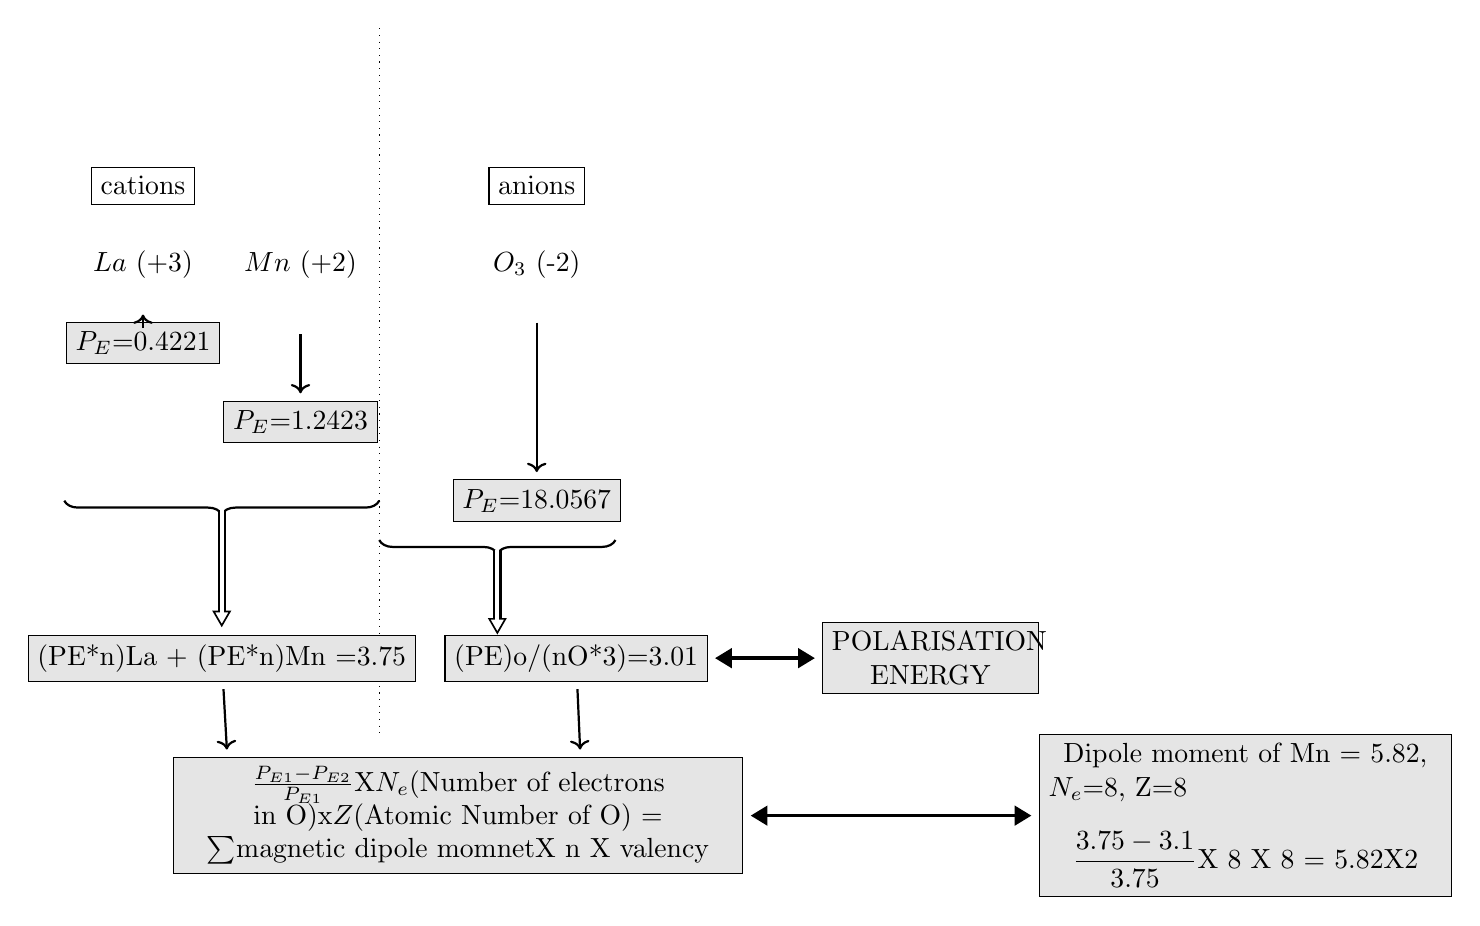
\begin{tikzpicture}
	%\draw node{cations};
	\node[rectangle,minimum size=0.01\textwidth,draw=black] (v1) at (0,0) {cations};
	\node[rectangle,draw=black] (v2) at (5,0) {anions};
	\node[circle] (E1) at (0,-1) {$La$ (+3)};
	\node[circle] (E2) at (2,-1) {$Mn$ (+2)};
	\node[circle] (E3) at (5,-1) {$O_3$ (-2)};
	
	\tikzstyle{edge}=[->,thick]
	\tikzstyle{arrow} = [ very thick, color=black, <->, >=Triangle]
	%\tikzstyle{line}=[draw,thick]
	%\tikzstyle{edge1}=[$\underbrace$,thick]
	\tikzstyle{block} = [draw,rectangle,fill=black!10,minimum size=0.005,outer sep=1mm,text centered,minimum height=2mm]
	%\node[rectangle](PE) at (0,-2) {$0.4221$};
	\node[block](PE1) at (0,-2) {$P_E$=0.4221};
	\node[block,text width=7cm](Dpe) at (4,-8){\normalsize{$\frac{P_{E1}-P_{E2}}{P_{E1}}$X$N_e$(Number of electrons in O)x$Z$(Atomic Number of O) =
	$\sum $magnetic dipole momnetX n X valency}};
\node[block,text width = 5cm](Dpe1) at (14,-8){Dipole moment of Mn = 5.82, $N_e$=8, Z=8
	\newline

	$\dfrac{3.75-3.1}{3.75}$X 8 X 8 = 5.82X2};
	\draw[arrow] (Dpe.east) to (Dpe1.west);
	\draw[edge](E1)--(PE1);
	\node[block,minimum size=1mm](PE2) at (2,-3) {$P_E$=1.2423};
	\draw[edge](E2)--(PE2);
	\node[block](PE3) at (5,-4) {$P_E$=18.0567};
	\draw[edge](E3)--(PE3);
	\node[block,text width=2.5cm](F4) at (10,-6) { POLARISATION ENERGY };
	%\node[below=1cm](E1) {La};
	%\node[below=1cm
	%\node[circle,draw=black] (v1) at (0,0) {La};
	%\tikzstyle{vertex} = [square]
	%\node[vertex](v2)at(2,0){Mn};
	%\draw[edge1](PE1)--(PE2);
	\draw[decorate,thick,decoration={brace,amplitude=5pt,mirror}] 
	(-1,-4) -- 
	(3,-4){}; 
	\draw (1,-4pt) coordinate (t_k)  {};
	\node(B1) at (1,-4){};
	\node(B2) at (4.5,-4.5){};
	\draw[dotted](3,2)--(3,-7);
	\draw[decorate,thick,decoration={brace,amplitude=5pt,mirror}] 
	(3,-4.5) -- 
	(6,-4.5){};
	\node[block,minimum size=1mm](F1) at (1,-6) {(PE*n)La + (PE*n)Mn  =3.75};
	\node[block,right of=F1](F2) at (4.5,-6) {(PE)o/(nO*3)=3.01};
	\tikzstyle{vecArrow} = [thick, decoration={markings,mark=at position
		1 with {\arrow[semithick]{open triangle 60}}},
	double distance=1.4pt, shorten >= 5.5pt,
	preaction = {decorate},
	postaction = {draw,line width=1.4pt, white,shorten >= 4.5pt}]
	\draw[vecArrow] (B1) to (F1);
	\draw[vecArrow] (B2) to (4.5,-5.7);
	\draw[arrow] (F2.east) to (F4.west);
	\draw[edge]([xshift=-4cm]F1) -- (Dpe);
		\draw[edge]([xshift=2.2cm]F2) -- (Dpe);
	%  \path{vecArrow}(F2)--(F4);
	%\framebox[0.5\textwidth][l]{n= (+3)     \hspace{1 cm}  (+2) \hspace{4 cm} (-2)} 
	%\framebox[0.5\textwidth][l]{La    \hspace{2 cm}  Mn \hspace{4 cm} $O_3$} 
	\end{tikzpicture}
\end{figure}	
%}

\begin{multicols}{2}
%\resizebox{250pt}{20pt}{
%	\begin{tabular}{|c|c|c|c|c|c|}
		%	\caption{MAGNETIC PARAMETRS f-shell}
%		\hline
%		n & $f_m$ & $\mu^{"} = \dfrac{2 n}{\pi}$ & $\chi_{V(c.g.s)}= \dfrac{\mu^{"}}{4 \pi}$ & \small{$\chi_{A(c.g.s)}= V_M*N_A*(\chi_v)$} &\small{ $\mu_s =  2.828 (\sqrt{{\chi_A T}}) $ B.M} \\
%		\hline
%		1.6 & 2.54 GHz &  1.0192 & $1.53X10^{3}$ & $2.32 X 10^{-3} $ & 2.53 B.M \\
%		\hline
%		2.1 & 7.7 GHz  & 1.3377 & $2.69 X 10^{-2}$ & $4.08 X 10^{-2}$ & 9.8 B.M \\
%		\hline
%	\end{tabular}
%}




%	\begin{tabular*}{0.5pt}{|c|c|c|c|c|}
%	\hline
%	\caption{MAGNETIC PARAMETRS d-shell}
%	$\mu$ & $ \mu^{''}$ & $\delta$ & $ \chi_m = \mu -1 $ & \tiny{$ \mu_J = \dfrac{1}{\mu_B} \sqrt{\frac{\chi_m ( 3kT)}{n_l \mu_o}}$}\\
%	\hline
%	1.032 & 269 &  3.4 & 0.032 &9.4 \\ 
%	\hline
%	2.57  & 20.59 & 2.34 & 1.57 & 2.53 \\ 
%	\hline
%\end{tabular*}



\subsection{Selection Criteria}

\begin{enumerate}
	\item{Derived Radius values: 
		The range of the upper and lower atomic radii serves as a criteria for material selection. It gives a broad idea for the suitability of different elements in the compound for a specified frequency. The derived radius values can be used to conclude the cation and the anion required for the MA by matching their atomic radii to the derived values}
	\item {$P_E $Effective energy  Parameter 
		After fulfilling above criteria the selected materials are then compared for the comptability based on the matching of the polarisation abilities. As shown in the flow chart for the compound ,both the cationic and the anionic sides of the compound are evaluated as per the given equation .
		\newline
		${\sum_{cations}} P_E $ X atom ratio X valency = $ \dfrac{P_{Eanion}}{valency \ X no \  of    \ atoms}$.}
%	\item{2.In case of mixed oxides , the mole fraction ratio of each cation or oxide compound can be derived as :-
%		CALCULATION FOR THE MOLAR RATIO :-
%		Depending on the ratio of the polarizability of the cation to anion , we can have the estimated molar fraction as
%		\begin{equation}
%		m = \frac{N_a X {r_a}^3}{N_c X {r_c}^3}
%		\end{equation}
		
%	}
\item{In case of mixed cations , the molar ratio of cation can be found by taking two cations at at time .Taking two cations a and b (with cation a radius larger than b) the molar ratio of cation a is given by :
	\normalsize{
${C_a} = \dfrac{r_{i_a} \ X \ P_{E_b} }{r_{i_b}\ X \ P_{E_a} }$ } and for cation b it is given by $C_b= 1 - C_a$ . If there are more than two cations involved, cation a , b, c(with atomic radii a$>$b$>$c) then cation b and c can be grouped together and evualte the above equation for cation a and b then for cation b and c separatley so that with molar ratio of cation a as $C_a$ , for b \Large{$C_{b_c}= 1-C_a$ and $C_b= C_{b_c} \ X \  \dfrac{r_{i_b} \ X \ P_{E_c} }{r_{i_c} \ X \ P_{E_b} }$ , further $C_c = C_{b_c} - C_b$.}}
	\item{In case of special crystal structures like pervoskite , spinel , fluorite , the radius ratio of the cation to anion has to be matched with the specified crystal requirement viz. }
\end{enumerate}
\subsection{ANALYSED AND SUGGESTED COMPOUNDS}
The methodoly explained above was verified by applying it  on some of the experimentally analysed microwave absorbing compounds.Based on that some of the compounds are also suggested as potential microwave aborbers for further study.
The compounds analysed here are oxides as in prevoskite structures, ferrites structures. Oxygen forms the anionic part whereas the cations can be mixed or single along with magnetic elements.
%\begin{table}
%	\centering
%	\caption{ANALYSED AND SUGGESTED COMPOUNDS}
%\textbf{
%\begin{table}[h]
%	\caption{Verified compounds as per the above method }
%\Large{

\captionof{table}{ Experimentally proven Compounds verified using the above methodology}

	\begin{tabular}{|c|}
	\hline
\textbf{	Analysed Compounds}  \\
\hline
	$La_0.8Ba_0.2Fe_xMn_{0.5(1-x)}Ti_{0.5(1-x)}O_3$ \cite{Adi}\\
	\hline
	$Ni_xFe_{3-x}O_4$ \cite{yunas2017magnetic} \\
	\hline
	$Ba_{(1-x)}Sr_xFe_2O_4$ \cite{Shukla} \\
	\hline
	$Ba_0.6Sr_0.4Fe_{12-z}Mn_zO19$ \cite{Adi} \\
	\hline
	$La_0.8Ca_{0.2-x}Ag_xMnO_3$ \cite{LaMn} \\
	\hline
	$LaNiO_3$ \cite{LNO}\\
	\hline
	
		\end{tabular}
%	}
%\end{table}
%\begin{table}[h]
	
%\caption{Suggested Compounds as per the above method}
%	\Large{
%\caption{th}
\captionof{table}{ {Compounds suggested using the above methodology}}
		\begin{tabular}{|c|}
			\hline
		\textbf{	Suggested Compounds}  \\
			\hline
			$Y_{2-x}Sr_xTi_2O_7$ \\
			\hline
			$La_0.8Er_0.15Ce_0.05TiO_3$ \\
			\hline
			$Zr_0.8Ce_0.2TiO_4$ \\
			\hline
			$GdMnO_3$ \\
			\hline
			$Er_{1-x}Nd_xxFe_12Co_xO_{19}$ \\
			\hline
			$DyNiO_3$ \\
			\hline
			
		\end{tabular}
%	}
%\end{table}
%\end{table}


% An example of a floating figure using the graphicx package.
% Note that \label must occur AFTER (or within) \caption.
% For figures, \caption should occur after the \includegraphics.
% Note that IEEEtran v1.7 and later has special internal code that
% is designed to preserve the operation of \label within \caption
% even when the captionsoff option is in effect. However, because
% of issues like this, it may be the safest practice to put all your
% \label just after \caption rather than within \caption{}.
%
% Reminder: the "draftcls" or "draftclsnofoot", not "draft", class
% option should be used if it is desired that the figures are to be
% displayed while in draft mode.
%
%\begin{figure}[!t]
%\centering
%\includegraphics[width=2.5in]{myfigure}
% where an .eps filename suffix will be assumed under latex, 
% and a .pdf suffix will be assumed for pdflatex; or what has been declared
% via \DeclareGraphicsExtensions.
%\caption{Simulation Results}
%\label{fig_sim}
%\end{figure}

% Note that IEEE typically puts floats only at the top, even when this
% results in a large percentage of a column being occupied by floats.


% An example of a double column floating figure using two subfigures.
% (The subfig.sty package must be loaded for this to work.)
% The subfigure \label commands are set within each subfloat command, the
% \label for the overall figure must come after \caption.
% \hfil must be used as a separator to get equal spacing.
% The subfigure.sty package works much the same way, except \subfigure is
% used instead of \subfloat.
%
%\begin{figure*}[!t]
%\centerline{\subfloat[Case I]\includegraphics[width=2.5in]{subfigcase1}%
%\label{fig_first_case}}
%\hfil
%\subfloat[Case II]{\includegraphics[width=2.5in]{subfigcase2}%
%\label{fig_second_case}}}
%\caption{Simulation results}
%\label{fig_sim}
%\end{figure*}
%
% Note that often IEEE papers with subfigures do not employ subfigure
% captions (using the optional argument to \subfloat), but instead will
% reference/describe all of them (a), (b), etc., within the main caption.




% Note that IEEE does not put floats in the very first column - or typically
% anywhere on the first page for that matter. Also, in-text middle ("here")
% positioning is not used. Most IEEE journals use top floats exclusively.
% Note that, LaTeX2e, unlike IEEE journals, places footnotes above bottom
% floats. This can be corrected via the \fnbelowfloat command of the
% stfloats package.



\section{Conclusion}
The theoritical model presented here gives an approach to predict the material composition for absorption applications. The method when applied to proven compositions gives an insight into their atomic level behaviours. Microwave  absorption is cumulative effect of different physical phenomenon which are realted to each other via energy conversion and dissipation. The idea suggested here will help in bringing out this complex relationship of the electrical, magnetic and atomic paarmeters and can benefit in forming new compostions. The compostions for multiple cations and anions can be predicted using the work here, which will enable formation of new , chemically stable,superior physical properties based absorbers . The mathematical model can also improve the industrial scaling for production of absorber panels on  a large level, as it can be integrated with the use automized manufacturing flow.




% if have a single appendix:
%\appendix[Proof of the Zonklar Equations]
% or
%\appendix  % for no appendix heading
% do not use \section anymore after \appendix, only \section*
% is possibly needed

% use appendices with more than one appendix
% then use \section to start each appendix
% you must declare a \section before using any
% \subsection or using \label (\appendices by itself
% starts a section numbered zero.)
%


%\appendices
%\section{Proof of the First Zonklar Equation}
%Appendix one text goes here.

% you can choose not to have a title for an appendix
% if you want by leaving the argument blank
%\section{}
%Appendix two text goes here.


% use section* for acknowledgement
%\section*{Acknowledgment}


%The authors would like to thank...


% Can use something like this to put references on a page
% by themselves when using endfloat and the captionsoff option.
\ifCLASSOPTIONcaptionsoff
\newpage
\fi



% trigger a \newpage just before the given reference
% number - used to balance the columns on the last page
% adjust value as needed - may need to be readjusted if
% the document is modified later
%\IEEEtriggeratref{8}
% The "triggered" command can be changed if desired:
%\IEEEtriggercmd{\enlargethispage{-5in}}

% references section

% can use a bibliography generated by BibTeX as a .bbl file
% BibTeX documentation can be easily obtained at:
% http://www.ctan.org/tex-archive/biblio/bibtex/contrib/doc/
% The IEEEtran BibTeX style support page is at:
% http://www.michaelshell.org/tex/ieeetran/bibtex/
\bibliographystyle{IEEEtran}
% argument is your BibTeX string definitions and bibliography database(s)
\bibliography{References}
%
% <OR> manually copy in the resultant .bbl file
% set second argument of \begin to the number of references
% (used to reserve space for the reference number labels box)
%\begin{thebibliography}{1}

%\bibitem{IEEEhowto:kopka}
%H.~Kopka and P.~W. Daly, \emph{A Guide to \LaTeX}, 3rd~ed.\hskip 1em plus
% 0.5em minus 0.4em\relax Harlow, England: Addison-Wesley, 1999.

%\end{thebibliography}

% biography section
% 
% If you have an EPS/PDF photo (graphicx package needed) extra braces are
% needed around the contents of the optional argument to biography to prevent
% the LaTeX parser from getting confused when it sees the complicated
% \includegraphics command within an optional argument. (You could create
% your own custom macro containing the \includegraphics command to make things
% simpler here.)
%\begin{biography}[{\includegraphics[width=1in,height=1.25in,clip,keepaspectratio]{mshell}}]{Michael Shell}
% or if you just want to reserve a space for a photo:

%\begin{IEEEbiography}{Michael Shell}
%Biography text here.
%\end{IEEEbiography}

% if you will not have a photo at all:
%\begin{IEEEbiographynophoto}{John Doe}
%Biography text here.
%\end{IEEEbiographynophoto}

% insert where needed to balance the two columns on the last page with
% biographies
%\newpage

%\begin{IEEEbiographynophoto}{Jane Doe}
%Biography text here.
%\end{IEEEbiographynophoto}

% You can push biographies down or up by placing
% a \vfill before or after them. The appropriate
% use of \vfill depends on what kind of text is
% on the last page and whether or not the columns
% are being equalized.

%\vfill

% Can be used to pull up biographies so that the bottom of the last one
% is flush with the other column.
%\enlargethispage{-5in}



% that's all folks
\end{multicols}
\end{document}
